\PassOptionsToPackage{dvipsnames}{xcolor}
\documentclass[hidelinks,a4paper,11pt]{book}
\usepackage[]{geometry}

\usepackage{ucs}
\usepackage[utf8]{inputenc}
\usepackage{amsmath}
\usepackage{amssymb}
\usepackage{siunitx}
\usepackage{cancel}
\usepackage[italian]{babel}
\usepackage{fontenc}
\usepackage{graphicx}
\graphicspath{{img/}}
\usepackage{circuitikz}
\ctikzset{
    resistors/scale=0.7,
    capacitors/scale=0.7,
    inductors/scale=0.7,
    sources/scale=0.7
    }

\usepackage{float}
\usepackage{xcolor}

\usepackage{hyperref}

\usepackage{arydshln} % dashed lines in matrix (array)


%Definizione 'globale' larghezza immagini
\newcommand{\picwid}{0.3\linewidth}

\date{28/11/21}
\title{Appunti Elementi di Automatica}
\author{Daniele Olivieri}
\begin{document}
\maketitle
\tableofcontents
%Lezione 01
\chapter{Introduzione}
L'automazione è una disciplina estremamente ampia, si intende in questo corso con
\textit{automazione} la progettazione, la realizzazione e la gestione di sistemi in grado di
eseguire dei compiti in maniera autonoma, senza l'intervento dell'uomo.

Nel corso verranno effettuate le analisi di sistemi dinamici, con un focus finale sulle analisi di
sistemi di controllo che verranno approfondite al corso di ``controlli''.

L'uomo ha sempre cercato di automatizzare i processi o i compiti che doveva eseguire, per ridurre
la fatica e l'usura per le attività manuali.

Un esempio è il \textbf{regolatore di Watt}, una macchina in grado di regolare il grado di
ammissione di una valvola di alimentazione per una macchina a vapore, al fine di mantenere costante
la velocità di rotazione della macchina.

Inizialmente l'operazione era compiuta da un operatore che regolava la temperatura della caldaia
fornendo più o meno combustibile.

Quest'oggetto racchiude l'essenza dei controlli automatici:
\begin{itemize}
 \item Elemento di trasduzione e misura, fondamentale per ottenere informazioni sulla grandezza da
controllare, in questo caso la velocità di rotazione delle macchine da controllare. L'uscita dello
strumento di misura può essere di diversa natura rispetto alla grandezza misurata ma comunque
proporzionale ad esso.
 \item Elemento di controllo (controllore), in questo caso il sistema di leve e pesi che varia la
posizione del cursore in funzione dell'input e delle sue caratteristiche come i pesi e le lunghezze
delle leve.
\item Attuatore, ossia uno strumento in grado di attuare la decisione del controllore sul sistema,
nel caso precedente la valvola.
\end{itemize}

Nel contesto più generale dei sistemi dinamici si riuscirà a modellare ed analizzare i sistemi
dinamici in generale e comprendere le proprietà fondamentali e strutturali dei sistemi studiati.

\section{Sistemi dinamici}
Un sistema è qualunque oggetto o processo materiale o immateriale, ben delimitato nel suo
funzionamento.
Potrebbe essere un sistema meccanico o termico, o ad esempio un sistema immateriale come
l'andamento del PIL in Italia.

Gli oggetti di interesse in particolare sono quelli \textit{dinamici}
che hanno ossia la possibilità di variare nel tempo alcune grandezze che li caratterizzano.

L'unica variabile indipendente considerata nell'intero corso sarà il tempo, anche i sistemi
astratti saranno comunque sistemi ``esistenti''.

33:04

%lezione_02.tex
\chapter{Modelli di sistemi dinamici}
I principali modelli di sistemi dinamici sono due:
\begin{itemize}
\item [$(IU)$]Ingresso-uscita
\begin{equation}
f\left(y^{(n)},y^{(n-1)},\ldots,y,u^{(m)},u^{(m-1)},\ldots,u\right)=0
\label{eq.:modello_ingresso_uscita}
\end{equation}
con $m<n$ (per la regola di Cauchy) per avere un sistema strettamente causale. Con $m=n$ un sistema
è causale ma non strettamente causale, in genere tutti i modelli fisici sono strettamente causali.
La \ref{eq.:modello_ingresso_uscita} prende il nome di \textit{equazione generale del sistema}
mentre $n$
prende il nome di \textit{ordine del sistema}.
La funzione può anche essere un sistema di equazioni differenziali di ordine inferiore.
\item[$(ISU)$] Ingresso-stato-uscita
\begin{equation}
y(t) = x_1(t), \dot{y}(t) = x_2(t),\ldots,y^{(n-1)}(t)=x_n(t)
\label{eq.:modello_ingresso_stato_uscita}
\end{equation}
Compaiono in questo modello tre tipologie di variabili, \textit{ingresso} e \textit{uscita} come nel
caso precedente e le variabili \textit{di stato} necessarie a completare il problema di Cauchy.
Un possibile insieme di variabili di stato sono quelle necessarie a specificare le condizioni
iniziali dell'equazione differenziale. Questo insieme può essere definito come \textit{stato} del
sistema.
Nella \ref{eq.:modello_ingresso_stato_uscita} si vede che il numero di variabili di stato $(x_n)$
necessarie alla risoluzione del problema è pari all'ordine del sistema.
\end{itemize}

Qualunque sistema dinamico può essere rappresentato con una diversa scelta delle variabili di
stato, varieranno le equazioni ma il modello resta valido per quel determinato sistema. La
rappresentazione ingresso-uscita è invece unica.

Si vede che nella rappresentazione $ISU$, una volta ottenuta l'equazione del sistema, questa può
essere trasformata per evidenziare particolari proprietà del sistema.

\newpage
\section{Costruzione di un modello ISU}
Si può costruire seguendo quattro passaggi
\begin{enumerate}
\item Scrivere tutte le equazioni del sistema (eq. diff.) conoscendo il modello fisico del sistema
\item Individuare le variabili d'ingresso e uscita, mediante il principio di causalità
\item Scegliere le variabili di stato dopo averne individuato il numero. Una scelta possibile è
quella mediante la regola di Cauchy
\item Riscrivere le equazioni di partenza trovate al punto uno nella seguente forma
\begin{equation}\left\{ \begin{aligned}
&\dot{x}_1 = f_1\left(x_1,\ldots,x_n,u_1,\ldots,u_m,t\right)\\
&\ \vdots \qquad \vdots\\
&\dot{x}_n = f_n\left(x_1,\ldots,x_n,u_1,\ldots,u_m,t\right)\\
&y_1 = g_1\left(x_1,\ldots,x_n,u_1,\ldots,u_m,t\right) \\
&\ \vdots \qquad \vdots\\
&y_n = g_n\left(x_1,\ldots,x_n,u_1,\ldots,u_m,t\right)
\end{aligned}\right.\qquad\text{ISU}
\label{eq.:ISU_generale}
\end{equation}
la $t$ in questo caso indica l'eventuale tempo varianza dei parametri del sistema e non la
dipendenza dal tempo delle variabili di stato (assunta vera implicitamente).
\end{enumerate}

\subsection{Costruzione modello ISU RLC}
Si considera l'esempio mostrato in figura \ref{Fig.:circuito_RLC}, analizzando l'equazione
\ref{eq.:ISU_generale} si vede che sono presenti $n$ equazioni differenziali di primo grado dato
che le funzioni $f$ e $g$ sono equazioni algebriche, non contengono termini differenziali.
Sono invece presenti $p$ equazioni puramente algebriche $g$ che legano lo stato, l'ingresso, il
tempo alle uscite.

\begin{enumerate}
\item Ricordando l'equazione del sistema ricavata in \ref{eq:equazione_RLC}
si formalizza il modello
\begin{equation}\left\{
\begin{aligned}
 e &= R i + L\dot{i} + \frac{q}{C}\\
 i &= \dot{q}
\end{aligned}\right.\end{equation}
\item Si individuano tutte le variabili: $e,i,q$

Si individuano dunque le variabili d'ingresso tra quelle con ordine di derivata più basso, in
questo caso la $e$ è differenziata zero volte, sarà un ingresso, in questo caso l'unico; le altre,
differenziate una volta, saranno le potenziali variabili di uscita.
\item Si scelgono le variabili di stato, si deve prima determinare l'ordine del sistema:\newline
\emph{il
numero di variabili di stato è pari alla somma del numero di volte che le variabili delle equazioni
compaiono differenziate tolte le variabili d'ingresso.}

Sommando l'ordine di derivazione di $i$ e $q$, variabili non d'ingresso si ottiene dunque $n=2$.

\item Si possono scegliere come variabili di stato tutte quelle che determinano le condizioni
iniziali, ossia\newline
\emph{tutte le variabili che compaiono differenziate e in numero pari al numero di volte
in cui viene differenziata.}

Per il sistema in esame
$$
x_1 = q,\quad x_2 = i
$$
\item Scrittura delle equazioni in forma ISU

$$
\left\{\begin{aligned}
\dot{x}_1 &= f_1\left(x_1,x_2,u\right) = \dot{q} = i = x_2\\
\dot{x}_2 &=f_2(x_1,x_2,u) = \dot{i} = \frac{e}{L} - \frac{R}{L}i-\frac{1}{LC}q =\\
&= -\frac{1}{LC}x_1 - \frac{R}{L}x_2 + \frac{1}{L}u\\
y_1 &= i = g_1(x_1,x_2,u)=x_2\\
y_2 &=q = g_2(x_1,x_2,u)=x_1
\end{aligned}\right.
$$
\end{enumerate}

\newpage
\section{Classificazione dei sistemi dinamici}
Per comodità si riporta la \ref{eq.:ISU_generale} in forma più compatta.
Si costruisce un vettore di variabili di stato, d'ingressi e di uscite
$$
x = \begin{bmatrix}
x_1\\
x_2\\
\vdots\\
x_n
\end{bmatrix} \in \mathbb{R}^n \textcolor{red}{\left(\in\mathbb{C}^n\right)}\
u=\begin{bmatrix}
u_1\\
u_2\\
\vdots\\
u_m
\end{bmatrix}\in\mathbb{R}^m\
y=\begin{bmatrix}
y_1\\
y_2\\
\vdots\\
y_p
\end{bmatrix}\in \mathbb{R}^p
$$
l'esistenza di variabili complesse per le variabili di stato è giustificata da scelte pratiche
utili alla risoluzione del problema anche se non legate strettamente a fenomeni fisici.

Di conseguenza la $f$ sarà un vettore di funzioni
$$\left.\begin{aligned}
&f_1\left(x_1,...,x_n,u_1,...,u_m,t\right)=f_1(x,u,t)\\
&\ \vdots\\
&f_n\left(x_1,\ldots,x_n,u_1,\ldots,u_m,t\right)=f_n(x,u,t)
\end{aligned}\right\} \Rightarrow f(x,u,t)=\begin{bmatrix}
f_1(x,u,t)\\
\vdots\\
f_n(x,u,t)
\end{bmatrix}
$$
Analogamente per le funzioni $g$
$$
\left.\begin{aligned}
&g_1(x,u,t)\\
&\ \vdots\\
&g_p(x,u,t)
\end{aligned}\right\}\Rightarrow
g(x,u,t) = \begin{bmatrix}
g_1(x,u,t)\\
\vdots\\
g_p(x,u,t)
\end{bmatrix}
$$

La forma generale della ISU diventa
\begin{equation}\text{ISU }\left\{
\begin{aligned}
\dot{x} = f(x,u,t)\\
y = g(x,u,t)
\end{aligned}\right.
\label{eq.:ISU_compatta}
\end{equation}

Si suppone che le funzioni $f,g$ siano lineari in $x$ e $u$ ossia che possano essere espresse come
combinazione lineare di quelle variabili $(x,u)$.

Ad esempio la funzione $f$
$$\begin{aligned}
&\dot{x}_1 = a_{11}(t)x_1+a_{12}(t)x_2 + \ldots + a_{1n}(t)x_n + b_{11}(t)u_1+\ldots+b_{1m}(t)u_m\\
&\ \vdots\\
&\dot{x}_n = a_{n1}(t)x_1 +  a_{n2}(t)x_2 + \ldots + a_{nn}(t)x_n + b_{n1}(t)u_1+\ldots+b_{nm}(t)u_m
\end{aligned}
$$

Analogamente la funzione $g$
$$\begin{aligned}
&g_1 = c_{11}(t)x_1 + \ldots + c_{1n}(t)x_n + d_{11}(t)u_1 + \ldots + d_{1m}(t)u_m\\
&\ \vdots\\
&g_p = c_{p1}(t)x_1 + \ldots + c_{pn}(t)x_n + d_{p1}(t)u_1+\ldots+d_{pm}(t)u_m
\end{aligned}$$

Si può scrivere il sistema in forma vettoriale ottenuto dal prodotto di un vettore riga contenente
i coefficienti e un vettore colonna contenente le variabili, questo per ogni elemento di
$\dot{x}$, si ottiene dunque una matrice $n\times n$ di coefficienti ed un vettore colonna di
variabili $x$.
$$\begin{aligned}
f = \dot{x} = A \cdot x + B\cdot u
\end{aligned}
$$
con
$$
A = \begin{bmatrix}
a_{11} & \dots & a_{1n} \\
\vdots & \ddots & \vdots \\
a_{n1} & \dots & a_{nn}
\end{bmatrix} \in \mathbb{R}^{n\times n} \quad
B = \begin{bmatrix}
b_{11} & \dots & b_{1m} \\
\vdots & \ddots & \vdots \\
b_{n1} & \dots & b_{nm}
\end{bmatrix} \in \mathbb{R}^{n\times m}
$$
La matrice $A$ è sempre quadrata mentre la matrice $B$ ha una dimensione che dipende dal numero di
ingressi e può diventare un vettore se l'ingresso è unico.

Si ripete la procedura per le funzioni $g$
$$
g = y = C\cdot x + D\cdot u
$$
con
$$
C = \begin{bmatrix}
c_{11} & \dots & c_{1n} \\
\vdots & \ddots & \vdots \\
c_{p1} & \dots & c_{pn}
\end{bmatrix} \in \mathbb{R}^{p\times n} \quad
D = \begin{bmatrix}
d_{11} & \dots & d_{1m} \\
\vdots & \ddots & \vdots \\
d_{p1} & \dots & d_{pm}
\end{bmatrix} \in \mathbb{R}^{p\times m}
$$
La matrice $D$ diventa uno scalare se il sistema ha un solo ingresso e una sola uscita.

Riassumendo
\begin{equation}
\text{ISU } \left\{\begin{aligned}
\dot{x} &= A(t)x + B(t) u \\
y &= C(t) x + D(t) u
\end{aligned}\right.
\label{eq.:ISU_compatta_matrice}
\end{equation}
\emph{Un sistema si dice \textbf{lineare} se le funzioni $f$ e $g$ sono entrambe lineari nello stato
e nell'ingresso},
ossia se possono essere scritte nella forma \ref{eq.:ISU_compatta_matrice}.

Se le equazioni del sistema compaiono nella seguente forma
$$\left\{\begin{aligned}
\dot{x} &= f(x,u)\\
y &= g(x,u)\end{aligned}\right.
$$
allora il sistema si dice \textit{stazionario} o \textit{tempo invariante},
ossia il sistema avrà sempre la stessa evoluzione fissato l'ingresso e lo stato iniziale. In caso
contrario il sistema si comporterebbe in maniera differente a seconda di quando viene
sollecitato e analizzato.
Se il sistema gode di entrambe le proprietà si dirà \textit{Lineare Tempo Invariante} e saranno
quelli prevalentemente analizzati nel corso, sono sempre risolvibili.
\newpage
\subsection{Ulteriori classificazioni}
Nel seguente sistema, l'uscita non dipende \textit{direttamente} dall'ingresso
$$
\left\{\begin{aligned}
\dot{x} &= f(x,u,t) \\
y &= g(x,t)
\end{aligned}
\right.
$$
viene definito \emph{sistema strettamente proprio}, in caso contrario è \emph{proprio}.

Nel caso di sistemi lineari
$$
\left\{
\begin{aligned}
\dot{x} &= Ax + Bu \\
y &= Cx
\end{aligned}
\right. \qquad D = 0 \Leftrightarrow \text{Strettamente proprio}
$$
In natura esistono solo sistemi strettamente propri, non esistono quelli propri,
qualunque ingresso ha bisogno di propagarsi nel sistema entro un certo tempo, non può quindi
modificare l'uscita istantaneamente.

\section{Sistemi elettrici}
Si richiamano le convenzioni utilizzate nei sistemi elettrici, saranno composti da uno o più
generatori di tensione o corrente e composti da bipoli passivi.

Verrà utilizzata la convenzione dell'utilizzatore per i seguenti bipoli
\begin{figure}[h]
\centering
\begin{circuitikz}
\draw (0,2) [R=$R$,i>^=$i$,v<=$v$] to (0,0);
\draw (1.5,1) node[label]{$v = Ri$};
\draw (4,2) [C=$C$,i>^=$i$,v<=$v$] to (4,0);
\draw (5.8,1) node[label]{$q = Cv$};
\draw (7.5,2) [L=$L$,i>^=$i$,v<=$v$] to (7.5,0);
\draw (9,1) node[label]{$\Phi = Li$};
\end{circuitikz}
\end{figure}

Derivando le equazioni dei bipoli dinamici rispetto al tempo si ottiene
$$\begin{aligned}
q &= Cv\stackrel{\frac{d}{dt}}{\rightarrow} \frac{dq}{dt} = i =
\frac{d}{dt} \left(Cv\right) \stackrel{C\text{ cost}}{=} C\frac{dv}{dt} = C\dot{v}\\
\Phi &= Li \stackrel{\frac{d}{dt}}{\rightarrow} \frac{d\Phi}{dt} = v = \frac{d}{dt}\left(Li \right)
\stackrel{L\text{ cost}}{=} L \frac{di}{dt} = L \dot{i}
\end{aligned}$$

Si aggiungono ai bipoli passivi i generatori di tensione e corrente
\begin{figure}[h]
\centering
\begin{circuitikz}[american voltages]
\draw (0,0) [european voltage source] to (0,2);
\draw (0.5,2) to [open, v^>=$ $,l=$e$] (0.5,0);
\draw (4,2) [current source,i<^=$i$] to (4,0);
\end{circuitikz}
\end{figure}

\subsection{Esempio rete RLC}
Si ha la seguente rete
\begin{figure}[h]
\centering
\begin{circuitikz}
\draw (0,0) to [voltage source,v=$e$]  (0,2)
            to [L=$L$,i>^=$i_L$,-*] (2,2)  node[above,label]{$A$}
            to [C,l_=$C$,i>_=$i_C$] (2,0)
            to (0,0);
\draw (2,2) to (3,2) to [R=$R$,i>^=$i_R$] (3,0) to (2,0);
\end{circuitikz}
\end{figure}

Si ricavano le equazioni del sistema utilizzando in questo caso le leggi di Kirchhoff applicate al
nodo $A$ e alla prima maglia (che comprende il generatore)
$$\left\{\begin{aligned}
i_L &= i_C + i_R &\Rightarrow&\ i_L = C\dot{v}_C + \frac{v_C}{R}\\
e &= v_L + v_C &\Rightarrow&\ e = L\dot{i}_L + v_C\\
v_C &= v_R
\end{aligned}\right.
$$

Elaborando le equazioni si vede che alcune variabili potranno risultare superflue, ad esempio in
questo caso $v_C$ e $v_R$ sono la stessa grandezza.

Si individuano ora le variabili e si dividono in ingressi e uscite al fine di rispettare il
principio di causalità ricordando che gli ingressi compaiono differenziati un numero minore di volte
$$\begin{matrix}
e& i_L& v_C\\
(0) & (1) & (1)\\
u & y & y\\
u & x_1 & x_2
\end{matrix}
$$

Si scelgono le variabili di stato, applicando la legge di Cauchy, il numero di ingressi è pari a
due perché entrambe le variabili compaiono differenziate una sola volta.
$$
n=2,\ x_1 = i_L,\ x_2 = v_C
$$

Si scrive quindi la ISU (il sistema è tempo invariante quindi le funzioni della ISU non dipendono
da $t$
$$\begin{aligned}
\dot{x}_1 &= f_1(x_1,x_2,u) = \dot{i}_L = \frac{e}{L} - \frac{v_C}{L} = -\frac{1}{L}x_2 +
\frac{1}{L} u\\
\dot{x}_2 &= f_2(x_1,x_2,u) = \dot{v}_C = \frac{i_L}{C} - \frac{v_C}{RC} = \frac{1}{C}x_1 -
\frac{1}{RC}x_2
\end{aligned}$$

Andrebbero aggiunte le relazioni che legano le uscite all'effettiva variabile di studio ad esempio
la tensione ai capi della resistenza e la corrente nell'induttanza, dunque
$$
y_1 = v_R,\ y_2 = i_L
$$
ma riferendosi al modello ISU
$$\begin{aligned}
y_1 &= g_1(x_1,x_2,\cancel{u}) = v_R = v_C = x_2\\
y_2 &= g_2(x_1,x_2,\cancel{u}) = i_L = x_1
\end{aligned}$$

Si vuole ora classificare la ISU, si verifica la linearità, tutte le funzioni $f$ e $g$ sono
lineari nello stato e negli ingressi, di conseguenza il sistema è lineare, è anche tempo invariante
dato che i parametri del sistema sono costanti nel tempo.

Si afferma ora che il sistema è strettamente proprio, ossia nell'espressione della $g$
non compare l'ingresso $u$.

Si riscrive il sistema in forma compatta utilizzando la notazione
\ref{eq.:ISU_compatta_matrice} ponendo
$$\begin{aligned}
x &= \begin{pmatrix}x_1\\x_2 \end{pmatrix},& u &= \begin{pmatrix} u \end{pmatrix},&
y&=\begin{pmatrix}
y_1 \\y_2 \end{pmatrix}\\
n&=2& m&=1&  p&=2
\end{aligned}
$$
dunque
\begin{equation}\left\{\begin{aligned}
&\dot{x} = \begin{bmatrix}
0 & -\frac{1}{L}\\
\frac{1}{C} & -\frac{1}{RC}
\end{bmatrix} x + \begin{bmatrix}\frac{1}{L}\\0 \end{bmatrix} u\\
&y =\begin{bmatrix}
0 & 1\\
1 & 0
\end{bmatrix} x + \begin{bmatrix}0\\0 \end{bmatrix}u
\end{aligned}\right.\end{equation}
\newpage

\subsection{Esempio rete RLC 2}
Si analizza il seguente circuito
\begin{figure}[h]
\centering
\begin{circuitikz}
\draw (0,0) to [current source,i=$i_1$] (0,2) to (2,2) node[above,label]{$A$}
            to [R=$R_1$,i>_=$i_{R_1}$,v<=$v_1$,*-] (2,0) to (0,0);
\draw (2,2) to (4,2) to [C=$C_1$,i>_=$i_{C_1}$] (4,0) to (2,0);
\draw (4,2) to [L=$L$,i>^=$i_L$] (6,2)
            to [C=$C_2$,i>^=$i_{C_2}$,v<=$v_{C_2}$] (6,0) to (4,0);
\draw (6,2) to (8,2) node[above,label]{$B$} to [R=$R_2$,i>^=$i_{R_2}$,*-] (8,0) to (6,0);
\draw (8,2) to (10,2) to [current source,i>^=$i_2$] (10,0) to (8,0);
\end{circuitikz}
\end{figure}

Applicando le leggi di Kirchhoff
$$\begin{aligned}
A: i_1 &= i_{R_1} + i_{C_1} + i_L\\
B: i_L &= i_{C_2} + i_{R_2} + i_2
\end{aligned}
$$
53:35

%Lezione 04

\subsection{Amplificatore operazionale}

Si introduce il modello dell'amplificatore operazionale, rappresentato da un
triangolo con tre morsetti, due in ingresso ed uno in uscita, quello con il
segno $-$ viene detto invertente, quello con il segno $+$ è non invertente.
Solitamente sono anche indicati i morsetti di alimentazione.
\begin{figure}[H]
 \centering
 \begin{circuitikz}
  \draw (0,0) node[op amp, anchor=-](OA){}
 (OA.+) -- ++(-1,0)
 to [short, -*] (-1,-1);
 \draw
(OA.-) -- ++(-1,0)
 to [short, -*] (-1,0);
 \draw (-1,-1) to [open,v^>=$e$] (-1,0);
 \draw (OA.out) -- ++(0,0) to [open,v^<=$v$,*-*] ++(0,-1)
  node[ground]{} ;
  \draw (OA.up)  node[vcc]{$+V_{cc}$};
  \draw (OA.down) node[vee]{$-V_{cc}$};
 \end{circuitikz}
\end{figure}
L'equazione caratteristica è
$$
v = -Ae
$$
Solitamente il valore $A$ è molto grande, anche \SI{e6}{} così come l'impedenza
d'ingresso tra i morsetti $+$ e $-$.

Dato un segnale in ingresso dunque, questo verrà restituito in uscita invertito
ed amplificato. Questa condizione è verificata se si suppone che la $v$ è
compresa tra i valori $[-V_{cc},+V_{cc}]$ di alimentazione.
In caso contrario l'uscita verrebbe ``tagliata'' e ci sarebbe un comportamento
non lineare, ipotesi di lavoro sempre evitata in questo corso.

Di conseguenza il segnale d'ingresso dovrebbe essere di valori pari a $v/A$,
valori bassissimi, si può ritenere dunque che la caduta di tensione
all'ingresso sarà prossima a \SI{0}{\volt}, è quindi come se l'ingresso fosse
un corto circuito (anche se non lo è).

L'impedenza d'ingresso, essendo di ordine elevato, implica che anche la
corrente nello stadio d'ingresso sia prossima a \si{0}, quindi si può modellare
come un circuito aperto.

In conclusione lo stadio d'ingresso si comporta sia da circuito chiuso che
circuito aperto e viene chiamato \textbf{corto circuito virtuale}.

Lo stadio d'uscita è confrontabile con un generatore ideale di tensione.

Si consideri il seguente circuito:
\begin{figure}[H]
\centering
\begin{circuitikz}
\draw (3,-.5) node[op amp](op){}
      (0,0) to [R=$R_1$,i=$i$,*-*]  (op.-)
            to ++(0,1)
            to [R=$R_2$,i>^=$i$] (4,1);
\draw (op.out) |- (4,1) ;
\draw (op.out) to [short,-*] ++(1,0)
                to [open,-*,v^<=$v$] ++(0,-0.5)
                node[ground]{};
\draw (op.+) to [short] ++(0,-.5)
        node[ground]{};
\draw (0,-1.5) node[ground]{} to [open,v^>=$e$,*-*] (0,0);
\end{circuitikz}
\end{figure}

Si ricorda che la tensione ai capi dell'ingressodell'amplificatore è nulla e la
corrente in ingresso lo è altrettanto.

Se si considera la maglia composta dal morsetto di uscita, la resistenza $R_2$
e il morsetto di ingresso si ottiene che la tensione ai capi di $R_2$ è pari a
$v$ ossia $v = -R_2i$.

Analogamente allo stadio d'ingresso, la tensione ai capi di $R_1$ è pari ad $e$
ossia $e = R_1i$.

Le due resistenze sono dunque attraversate dalla stessa corrente $i$.

Sostituendo le due equazioni precedenti si ottiene la tensione in uscita in
funzione di quella in ingresso
\begin{equation}
v = -R_2 i = -\frac{R_2}{R_1}e
\label{eq.:amplificatoreOperazionale}
\end{equation}

Si può variare dunque il guadagno dell'amplificatore variando opportunamente il
rapporto tra le resistenze.
Collegando un secondo amplificatore in cascata con guadagno $-1$ si ottiene una
tensione finale concorde a quella in ingresso. Questo secondo elemento viene
definito \textit{buffer}.
Il \textit{buffer} è molto utile per disaccoppiare i circuiti.

\subsection{Circuito integratore}
Si analizza il seguente circuito
\begin{figure}[H]
\centering
\begin{circuitikz}
\draw (3,-.5) node[op amp](op){}
      (0,0) to [R=$R$,i=$i$,*-*]  (op.-)
            to ++(0,1)
            to [C=$C$,i>^=$i$,v<=$v_C$] (4,1);
\draw (op.out) |- (4,1) ;
\draw (op.out) to [short,-*] ++(1,0)
                to [open,-*,v^<=$v$] ++(0,-0.5)
                node[ground]{};
\draw (op.+) to [short] ++(0,-.5)
        node[ground]{};
\draw (0,-1.5) node[ground]{} to [open,v^>=$e$,*-*] (0,0);
\end{circuitikz}
\end{figure}
A differenza del circuito precedente il sistema è dinamico, se ne ricava di
seguito la ISU.

Equazioni caratteristiche
\begin{equation}\left\{\begin{aligned}
v &= -v_C \\
i &= \frac{e}{R} = C \dot{v}_C
\end{aligned}\right.\Rightarrow
e=-RC\dot{v}
\label{eq.:differenzialeIntegratore}
\end{equation}

Si analizzano le variabili seguendo la regola di causalità

$$
\begin{matrix}
 e    & v \\
 (0)  &(1) \\
 u    & x
 \end{matrix}
$$

L'ordine del sistema è unitario dunque il modello ISU non sarà un'equazione
matriciale
$$
\left\{\begin{aligned}
        \dot{x} &= \dot{v} = -\frac{1}{RC} u \\
        y & = v = x
       \end{aligned}\right.
$$
Il sistema è lineare tempo invariante strettamente causale (o proprio LTISP).
Se si integra la \ref{eq.:differenzialeIntegratore} si ottiene
$$
v(t) = v(t_0) - \frac{1}{RC}\int_{t_0}^{t} e(\tau)d\tau
$$
Ossia l'uscita, a meno di un fattore di guadagno è l'integrale dell'ingresso,
si è realizzato un circuito integratore ideale.

\subsubsection{Circuito integratore reale}
Si inserisce in parallelo alla capacità del circuito precedente una resistenza
di scarica parassita $R_s$.

\begin{figure}[H]
\centering
\begin{circuitikz}[smallR/.style={R, resistors/scale=0.5}]
\draw (3,-.5) node[op amp](op){}
      (0,0) to [R=$R$,i=$i$,*-*]  (op.-)
            to ++(0,1)
            to [C=$C$,i>^=$i_C$,v<=$v_C$] (4,1)
            -- ++(0,1) to [smallR,l_=$R_s$,i_<=$i_{R_s}$] ++(-2.1,0) -|
++(0,-1);
\draw (op.out) |- (4,1) ;
\draw (op.out) to [short,-*] ++(1,0)
                to [open,-*,v^<=$v$] ++(0,-0.5)
                node[ground]{};
\draw (op.+) to [short] ++(0,-.5)
        node[ground]{};
\draw (0,-1.5) node[ground]{} to [open,v^>=$e$,*-*] (0,0);
\end{circuitikz}
\end{figure}

Le equazioni del sistema saranno
$$\left\{\begin{aligned}
          v &= -v_C \\
          i &= \frac{e}{R} = C\dot{v}_C + \frac{v_C}{R_s}
         \end{aligned}\right.\Rightarrow
e = -RC\dot{v} - \frac{R}{R_s}v
$$
Si riscrivono le variabili
$$
\begin{matrix}
 e    & v \\
 (0)  &(1) \\
 u    & x
 \end{matrix}
$$
la ISU
$$\left\{\begin{aligned}
\dot{x} &= \frac{1}{R_sC}x - \frac{1}{RC}e\\
y & = v = x
\end{aligned}\right.
$$
È presente un termine aggiuntivo rispetto al precedente sistema.
Se $R_s$ fosse una vera capacità parassita, ossia molto più grande di $R$, si
trascurerebbe il primo termine dell'equazione ritornando al caso precedente; in
caso contrario si è in presenza di un integratore \textit{reale}, governato
ossia da una costante di tempo che ne indica la velocità di scarica.

\newpage
\subsection{Circuito derivatore}
Si invertono in questo circuito la posizione del condensatore e della
resistenza, si suppone inoltre di alimentare il circuito con un generatore
ideale di tensione.
\begin{figure}[H]
\centering
\begin{circuitikz}
\draw (3,-.5) node[op amp](op){}
      (0,0) to [C=$C$,i=$i$,v_<=$e$,*-*]  (op.-)
            to ++(0,1)
            to [R=$R$,i>^=$i$,v<=$v_R$] (4,1);
\draw (op.out) |- (4,1) ;
\draw (op.out) to [short,-*] ++(1,0)
                to [open,-*,v^<=$v$] ++(0,-0.5)
                node[ground]{};
\draw (op.+) to [short] ++(0,-.5)
        node[ground]{};
\draw (0,-1.5) node[ground]{} to [open,v^>=$e$,*-*] (0,0);
\end{circuitikz}
\end{figure}

Si scrivono le equazioni
$$
v = -Ri = -RC \dot{e}
$$
il circuito è un derivatore ideale.
In questo caso ideale, il sistema è non causale, dovrebbe fornire in uscita la
derivata del segnale in ingresso.

Sviluppando l'analisi
$$
\dot{e} = -\frac{1}{RC}v
$$
$$
\begin{matrix}
 \dot{e} & v\\
 (1) & (0)
\end{matrix}
$$
seguendo le regole precedenti si direbbe che la variabile causa è la $v$ mentre
l'effetto è la $e$, ciò è in contrasto con l'evidenza fisica del sistema.

La regola di Cauchy non vale per i sistemi non causali.
Si sta affermando che il generatore possa pilotare istantaneamente una capacità.

Per modellare un sistema analogo va inserita nel circuito una resistenza $R_s$
in serie al generatore di tensione (o analogamente alla porta d'ingresso).
\begin{figure}[H]
\centering
\begin{circuitikz}[smallR/.style={R, resistors/scale=0.5}]
\draw (3,-.5) node[op amp](op){}
      (-2,0) to [smallR,l=$R_s$] ++(2,0) to [C=$C$,i=$i$,v_<=$v_C$,*-*]  (op.-)
            to ++(0,1)
            to [R=$R$,i>^=$i$,v<=$v_R$] (4,1);
\draw (op.out) |- (4,1) ;
\draw (op.out) to [short,-*] ++(1,0)
                to [open,-*,v^<=$v$] ++(0,-0.5)
                node[ground]{};
\draw (op.+) to [short] ++(0,-.5)
        node[ground]{};
\draw (-2,-1.5) node[ground]{} to [open,v^>=$e$,*-*] (-2,0);
\end{circuitikz}
\end{figure}
Le equazioni del sistema:
$$\left\{\begin{aligned}
v &= -Ri = -RC\dot{v}_C\\
e &= R_s i + v_C \Rightarrow i = \frac{e-v_C}{R_s}
\end{aligned}\right.$$

Ricavando la $i$ dalla seconda e sostituendo nella prima
$$
\dot{v}_C =
\frac{1}{\cancel{R}C}\left(\frac{\cancel{R}}{R_s}\left(e-v_C\right)\right) =
\frac{e-v_C}{R_sC}
$$
Si analizzano le variabili
$$\begin{matrix}
e & v_C \\
(0) & (1) \\
u & x
\end{matrix}$$

dunque l'equazione del sistema del primo ordine
$$\left\{\begin{aligned}
\dot{x} &= \frac{u}{R_sC} - \frac{x}{R_sC}\\
y &= v = -Ri = \frac{R}{R_s}u - \frac{r}{R_s}x
\end{aligned}\right.$$
Il sistema è dunque lineare tempo invariante causale ma non strettamente
causale.

\newpage
\section{Sistemi meccanici}
Si vogliono analizzare gli elementi principali dei sistemi meccanici.
\subsubsection{Moti lineari}
Si considerano inizialmente i sistemi governati da moti lineari.
Gli elementi principali sono:
\begin{itemize}
 \item Elemento \textbf{massa}: $m$ rappresentato solitamente con un cubetto o
una sfera, se sulla massa sono applicate $n$ forze $f_n$, questa potrà muoversi
solo lungo una direzione nello spazio e si indica con $s$ la variabile di
spostamento. Per convenzione la forza è positiva se concorde al verso positivo
degli spostamenti. L'oggetto subirà un'accelerazione pari a
$$
m\ddot{s} = \sum_n f_n
$$

\item Elemento \textbf{molla}: $k$ è il coefficiente elastico della molla,
determina la forza che la molla esplica proporzionale alla sua deformazione
rispetto alla condizione di riposo e in verso opposto (forza di richiamo).
I due estremi della molla devono essere indicati nel sistema di riferimento,
dunque
$$
f = k(s_2-s_1)
$$
Si assume con $s_2=s_1$ la condizione di riposo. Se la molla viene estesa, la
differenza $s_2-s_1$ è positiva e la molla esplica una forza verso il suo
interno, viceversa se viene compressa $s_2-s_1$ è negativo e la forza è verso
l'esterno; ciò è vero per tutte le molle reali che hanno coefficiente elastico
positivo.

\item Elemento \textbf{smorzatore viscoso}: $b$ è il coefficiente di attrito
viscoso, anch'esso esplica una forza positiva verso il suo interno e si
considerano le velocità $\dot{s}_1$ e $\dot{s}_2$ dei suoi estremi.
La forza esplicata dallo smorzatore è dunque proporzionale alla velocità
relativa dei suoi estremi
$$
f = b(\dot{s}_2-\dot{s}_1)
$$
Anche in questo caso la forza è sempre opposta al verso di movimento per gli
smorzatori reali con $b$ positiva.
\end{itemize}

Se il sistema ha più gradi di libertà deve essere fornita un'equazione per ogni
possibile direzione.

\newpage
\subsubsection{Moti rotazionali}
Esiste una perfetta simmetria tra le due tipologie di moti, a patto di fornire
le giuste equivalenze
\begin{itemize}
 \item Elemento \textbf{inerzia}: definito un asse, si definisce con $J$ il
parametro che determina l'attitudine del corpo a generare accelerazioni
angolari. Si applicano una serie di $n$ coppie $\tau_n$ all'oggetto, positive
se concordi all'angolo $\theta$; il corpo si metterà in rotazione con una
certa inerzia
$$
J\ddot{\theta} = \sum_n \tau_n
$$

$\theta$ è l'angolo di cui è ruotato l'asse, dunque $\ddot{\theta}$ è
l'accelerazione angolare.

 \item Elemento \textbf{molla rotazionale}: analogamente alla molla lineare, la
molla rotazionale esplica una forza proporzionale alla rotazione relativa dei
suoi due assi. $\theta_1$ e $\theta_2$ sono le posizioni dei due assi, la
costante della molla è ancora $k$, la coppia di richiamo $\tau$ si pone
concorde a $\theta_1$ e discorde a $\theta_2$ dunque:
$$
\tau = k\left(\theta_2 - \theta_1\right)
$$

 \item Elemento \textbf{smorzatore viscoso rotazionale}: sono presenti due assi
e si indica con $\dot{\theta}_1$ la velocità angolare del primo asse e
$\dot{\theta}_2$ quella del secondo. La coppia $\tau$ sarà concorde alla
velocità $\theta_1$ e discorde a $\theta_2$. Se $b$ è il coefficiente viscoso
allora la coppia sarà
$$
\tau = b(\dot{\theta}_2 - \dot{\theta}_1)
$$
\end{itemize}

È importante mantenere la coerenza nelle convenzioni.

\newpage
\subsection{Esempio sistema Massa-Molla-Smorzatore}
Si suppone di avere un carrello di massa $m$ al quale viene applicata una forza
$f$. Il carrello è vincolato alla parete mediante una molla di costante $k$ e
uno smorzatore di coefficiente $b$.
\begin{figure}[h]
 \centering
 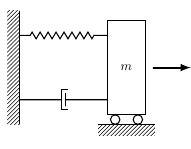
\includegraphics[width=\picwid]{massa_molla_smorzatore_HQ}
 % massa_molla_smorzatore_HQ.png: 0x0 px, 0dpi, 0.00x0.00 cm, bb=
 \label{fig:massa_molla_smorzatore_HQ}
\end{figure}

Si vuole costruire il modello ISU dell'oggetto.
Il corpo ha un solo grado di libertà, si fissa un sistema di riferimento.
Si indica con $s$ la posizione dell'oggetto.

Esistono due modalità principali per scrivere le equazioni di un sistema
meccanico, l'approccio Newtoniano e l'approccio Lagrangiano, si usa in seguito
quello Newtoniano.

Si applica il secondo principio delle dinamica, ossia le formule
precedentemente analizzate.

$$
m\ddot{s} = f - ks - b\dot{s}
$$
$(s_1 , \dot{s}_1 = 0)$

Il numero di equazioni da scrivere è pari al numero di masse moltiplicate per i
rispettivi gradi di libertà.

Le variabili del sistema sono
$$\begin{matrix}
f & s \\
(0) & (2) \\
f & s & \dot{s}\\
u & x_1 &x_2
\end{matrix}$$

Il sistema è del secondo ordine.
$$\left\{\begin{aligned}
\dot{x}_1 &= \dot{s} = x_2 \\
\dot{x}_2 &= \ddot{s} = \frac{1}{m}f - \frac{k}{m}s - \frac{b}{m}s =
-\frac{k}{m}x_1 - \frac{b}{m}x_2 + \frac{1}{m}u
\end{aligned}\right.$$

Le uscite saranno assegnate arbitrariamente, il sistema è lineare
tempo invariante e strettamente causale.


\subsection{Esempio Massa-Molla-Smorzatore con due masse}
Si vuole analizzare il modello ISU del seguente sistema composto da due masse
disposte nel seguente modo:
\begin{figure}[h]
 \centering
 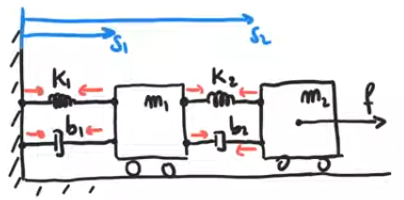
\includegraphics[width=\picwid]{massa_molla_smorzatore_esempio_2.png}
 \label{fig:massa_molla_smorzatore_esempio_2}
\end{figure}

Si individua il sistema di riferimento e si indica con $s_1$ la posizione della
prima massa ed $s_2$ la seconda.
Esiste un'unica direzione di movimento e sono presenti due masse, dunque si
scriveranno due equazioni.
$$\left\{\begin{aligned}
m_1\ddot{s}_1 &= k_2(s_2-s_1) + b_2(\dot{s}_2-\dot{s}_1) -k_1s_1 - b_1\dot{s}_1
\\
m_2\ddot{s}_2 &= f - k_2(s_2-s_1) - b_2(\dot{s}_2-\dot{s}_1)
\end{aligned}\right.$$

Si analizzano le variabili del sistema
$$\begin{matrix}
f & s_1& \dot{s}_1 & s_2 &\dot{s}_2 \\
(0) & (2) & & (2) \\
u & x_1 & x_2 & x_3 & x_4
\end{matrix}$$

L'ordine del sistema è dunque quattro $(n=4)$, dato che ogni variabile non di
ingresso viene differenziata due volte.

Si riscrivono le equazioni in forma ISU
$$\left\{\begin{aligned}
\dot{x}_1 &= \dot{s}_1 = x_2 \\
\dot{x}_2 &= \ddot{s}_1 = \frac{k_2}{m_1}(x_3-x_1) + \frac{b_2}{m_1} (x_4-x_2)
- \frac{k_1}{m_1}x_1 - \frac{b_1}{m_1}x_2\\
\dot{x}_3 &=\dot{s}_2 = x_4 \\
\dot{x}_4 &= \ddot{s}_2 = \frac{1}{m_2}u -\frac{k_2}{m_2}(x_3-x_1) -
\frac{b_2}{m_2}(x_4 - x_2)\\
\ &\text{Uscite assegnate}\\
y_1 &= s_1 = x_1 \\
y_2 &= s_2 = x_3
\end{aligned}\right.$$

\newpage
Il sistema è lineare tempo invariante strettamente causale, si può porre il
sistema in forma matriciale compatta
$$x =
\begin{pmatrix}
 x_1 \\ x_2 \\ x_3 \\ x_4
\end{pmatrix} \quad
y= \begin{pmatrix}
    y_1 \\ y_2
   \end{pmatrix}
$$
$$\text{ISU} = \left\{\begin{aligned}
\dot{x} &= \begin{pmatrix}
0 & 1 & 0 & 0 \\
\\
-\frac{k_1+k_2}{m_1} & -\frac{b_1+b_2}{m_1} &
\frac{k_2}{m_1} & \frac{b_2}{m_1}\\
\\
0 & 0 & 0 & 1\\ \\
\frac{k_2}{m_2} & \frac{b_2}{m_2} & -\frac{k_2}{m_2} & -\frac{b_2}{m_2}
          \end{pmatrix}x +
          \begin{pmatrix}
        0 \\ 0 \\ 0 \\ \frac{1}{m}
          \end{pmatrix}u\\
y &=      \begin{pmatrix}
           1 & 0 & 0 & 0 \\
           0 & 0 & 1 & 0
          \end{pmatrix}x
\end{aligned}\right.$$
27:58


\section{Sistemi termici}
Al fine di descrivere i sistemi termici è fondamentale conoscere l'equazione
del bilancio termico.

Si considera un certo volume di superficie $S$ caratterizzato da un unico
parametro: la \textit{capacità termica}; la capacità termica di un corpo è
l'attitudine del corpo a modificare la sua temperatura quando questo viene
investito da una certa potenza termica.

È inoltre esprimibile come il rapporto tra il calore entrante nel corpo e la
variazione di temperatura che esso subisce, è considerata un'inerzia termica.
Il volume può interagire con l'ambiente che lo circonda mediante la superficie
$S$, quest'ultima consente di realizzare gli scambi di potenza termica.
%Posizione della figure non specificata, [h] missing
% è una prova dell'impaginamento automatico di LaTex
\begin{figure}
 \centering
 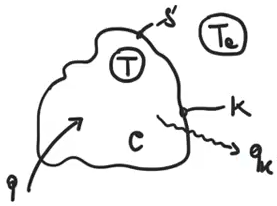
\includegraphics[width=\picwid]{corpo_termico.png}
 % corpo_termico.png: 277x206 px, 96dpi, 7.33x5.45 cm, bb=0 0 208 154
 \label{Fig.:corpo_termico}
\end{figure}

Si suppone inoltre che il corpo abbia una temperatura uniforme $T$, costante in
ogni suo punto, l'ambiente esterno invece sarà ad una temperatura $T_a\neq T$.

La differenza tra le due temperature genererà dei flussi di potenza termica dal
corpo (o ambiente) più caldo a quello più freddo.
La quantità di energia termica che attraversa la superficie dipenderà dalla
superficie stessa e in particolare dalla sua \textit{resistenza termica}.

Si indica con $K$ il coefficiente di scambio termico che la superficie consente
di sviluppare.
Il flusso termico $q_K$ è definito per convenzione positivo se uscente dal
corpo, dunque
$$
q_K = K(T-T_a)
$$

Si riportano le equazioni di bilancio termico che interessano il volume se
questo è sottoposto ad $n$ flussi termici $q_n$ ed $i$ superfici di scambio
termico con coefficiente di scambio $K_i$ e con ambienti a temperature $T_i$
(diverse o meno fra loro):
\begin{equation}
C\dot{T} = \sum_n q_n -\sum_i K_i(T-T_i)
\label{eq.:bilancio_termico}
\end{equation}

Si riporta il modello ISU del sistema in esame con una sola potenza termica in
ingresso ed un solo scambio termico con un unico ambiente
 a temperatura $T_a$
$$
C\dot{T} = q -K(T-T_a)
$$
variabili:
$$\begin{matrix}
q & T_a & T \\
(0) & (0) & (1) \\
u_1 & u_2 & x
\end{matrix}
$$
\emph{Attenzione, $T_a$ è a tutti gli effetti una variabile di ingresso, anche
se resta costante, si parla di ingresso non manipolabile}

Equazioni del sistema:
$$\left\{\begin{aligned}
\dot{x} &=  \dot{T} = \frac{1}{C}u_1-K(x-u_2) \\
y &= T = x
\end{aligned}\right.$$

\subsection{Esempio forno elettrico}
Dato un volume chiuso si indica con $C_1$ la sua capacità termica e $T_1$ la
sua temperatura.
Si suppone che sia presente attorno al volume una parete con capacità termica
$C_2$ ed una temperatura supposta uniforme $T_2$, l'ambiente esterno è alla
temperatura $T_a$.
All'interno del volume è presente una resistenza elettrica che fornisce una
certa potenza termica $q$.

\begin{figure}[h]
 \centering
 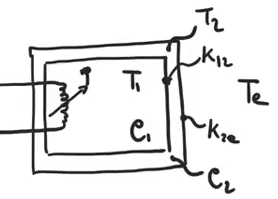
\includegraphics[width=\picwid]{forno_elettrico.png}
 % forno_elettrico.png: 278x199 px, 96dpi, 7.35x5.26 cm, bb=0 0 208 149
 \label{Fig.:forno_elettrico}
\end{figure}

Attraverso la parete, la temperatura è in realtà un gradiente termico e non
uniforme.
Si indicano con $K_{12}$ e $K_{2a}$ i coefficienti di scambio termico tra le
rispettive superfici.

Per ogni volume con una certa capacità termica, va scritta un'equazione del
bilancio
$$\left\{\begin{aligned}
C_1\dot T_1 &= q - K_{12}(T_1-T_2)\\
C_2\dot{T}_2 &= -K_{12}(T_2-T_1) - K_{2a}(T_2-T_a)
\end{aligned}\right.$$
Si nota come il flusso termico $K_{12}(T_1-T_2)$ uscente dal primo volume sia
entrante nel secondo.
Utilizzando sempre la stessa convenzione sui versi non si commettono errori e
non bisogna riflettere sui versi effettivo dei flussi termici.

Variabili:
$$\begin{matrix}
q & T_a & T_1 & T_2 \\
(0) & (0) & (1) & (1) \\
u_1 & u_2 & x_1 & x_2
\end{matrix}$$
Il sistema è di ordine due.

$$\left\{\begin{aligned}
\dot x_1 &= \dot{T}_1 = \frac{1}{C_1}u_1 - K_{12}(x_1-x_2)\\
\dot x_2 &= \dot T_2 = -\frac{K_{12}}{C_2} (x_2-x_1) -
\frac{K_{2a}}{C_2}(x_2-u_2)\\
y_1 &= T_1 = x_1 \\
y_2 &= T_2 = x_2
\end{aligned}\right.$$

Se si indica con $v$ la tensione ai capi della resistenza $R$, la potenza
termica si sarebbe potuta esprimere come $q=\frac{v^2}{R}$ e se si fosse scelta
$v$ come ingresso si avrebbe avuto un termine al quadrato
$$
\dot x_1 = \dot T_1 = \frac{1}{C_1 R} u_1^2 - K_{12}(x_1-x_2) \dots
$$
Lo stesso sistema, con variabili diverse sarebbe diventato non lineare.

\section{Sistemi idraulici}
Un sistema idraulico è modellabile come un serbatoio in grado di contenere un
certo liquido. Si suppone che ci sia la possibilità di aggiungere una certa
quantità di liquido $q_i$.

Si suppone che la sezione del serbatoio sia regolare ed $h$ l'altezza del
liquido nel serbatoio. Si suppone che sia presente una valvola in uscita in
grado di prelevare un flusso di liquido in uscita $q_u$, analogamente con una
valvola in ingresso.

\begin{figure}[h]
 \centering
 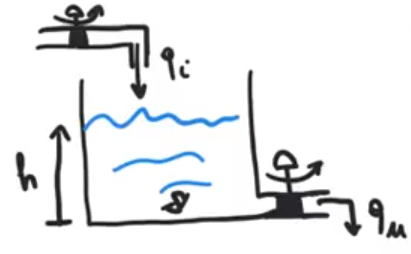
\includegraphics[width=\picwid]{serbatoio_due_valvole.png}
 % serbatoio_due_valvole.png: 411x254 px, 96dpi, 10.87x6.72 cm, bb=0 0 308 190
 \label{Fig.:serbatoio_due_valvole}
\end{figure}


Il flusso di un liquido viene chiamato \textbf{portata} e ci si può
riferire
ad una portata \textit{massica} ($w$) [\si{\kilogram/\second}]
 o \textit{volumetrica} ($q$) $\si{\meter^3/\second}$, con la seguente
relazione che le lega
$$
w = \rho q
$$
dove $\rho$ è la \textit{densità} del liquido.

È fondamentale considerare i liquidi incomprimibili, ossia che la sua densità
resti costante affinché si possa sempre utilizzare l'uno o l'altro riferimento.
Ci si riferirà generalmente alla portata volumetrica.

La quantità di massa nel serbatoio è pari alla differenza di massa entrante e
uscente, supposta la densità costante invece si può quindi ragionare sui volumi
e le $j$ portate entranti e $k$ portate uscenti ossia:
$$
\dot{V} = \frac{d}{dt}(S\cdot h) = S\dot{h} = \sum_j q_i - \sum_k q_u
$$
con $\dot{V}$ la variazione di volume e $S$ la sezione del serbatoio
assunta costante (altrimenti $S\dot h + \dot{S}h$).

Per il sistema in esame con un ingresso ed un'uscita si ha
$$
\dot{V} = q_i - q_u
$$
Si suppone che la valvola in uscita sia autoregolata, la portata di un fluido
attraverso una valvola dipende sia dalla sua sezione regolabile che dalla
differenza di pressione a monte e a valle della stessa, funzione dell'altezza
del fluido.

Un modello semplice di valvola ammette un parametro $a$ che
indica il grado di apertura della valvola ed esprime la portata con la
seguente
$$
q = a\sqrt{h}
$$

Si scrive il modello ISU, l'equazione è già stata ricavata, si procede con le
variabili:
$$
\begin{matrix}
q_i & h \\
(0) & (1) \\
u & x
\end{matrix}
$$

$$\left\{\begin{aligned}
\dot{x} &= \dot{h} = \frac{1}{S} u - \frac{a}{S}\sqrt{x} \\
y &= V = Sh = Sx
\end{aligned}\right.$$
Il sistema è non lineare e strettamente proprio.

\subsection{Sistema idraulico con due serbatoi}
Si ha un sistema formato da due serbatoi in cascata con un flusso
monodirezionale tra l'uscita di uno e l'ingresso dell'altro.
\begin{figure}[h]
 \centering
 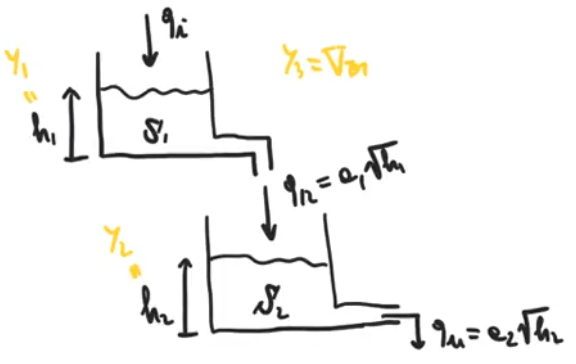
\includegraphics[width=\picwid]{doppio_serbatoio.png}
 % doppio_serbatoio.png: 576x364 px, 96dpi, 15.24x9.63 cm, bb=0 0 432 273
 \label{Fig.:doppio_serbatoio}
\end{figure}

Si indica con $h_1$ l'altezza di liquido nel serbatoio di sezione $S_1$ ed
$h_2$ l'altezza nel serbatoio di sezione $S_2$. Le portate in uscita dai due
serbatoi saranno:
$$\begin{aligned}
q_{12} &= a_1\sqrt{h_1} //
q_u &= a_2\sqrt{h_2}
\end{aligned}$$

Le equazioni del sistema saranno:
$$\left\{\begin{aligned}
S_1\dot h_1 &= q_i - q_{12} = q_i - a_1\sqrt{h_1} \\
S_2 \dot h_2 &= q_{12} - q_u = a_1\sqrt{h_1} - a_2\sqrt{h_2}
\end{aligned}\right.$$

Si analizzano le variabili
$$\begin{matrix}
q_i & h_1 & h_2 \\
(0) & (1) & (1) \\
u & x_1 & x_2
\end{matrix}$$

Il sistema di ordine due in forma ISU
$$\left\{\begin{aligned}
\dot x_1 &= \dot h_1 = \frac{1}{S_1} u - \frac{a_1}{S_1} \sqrt{x_1} \\
\dot x_2 &= \dot h_2 = \frac{a_1}{S_2}\sqrt{x_1} - \frac{a_2}{S_2} \sqrt{x_2} \\
y_1 &= h_1 = x_1 \\
y_2 &= h_2 =x_2 \\
y_3 &= V_{\text{tot}} = S_1h_1 + S_2h_2 = S_1x_1 + S_2 x_2
\end{aligned}\right.$$

Il sistema è non lineare strettamente proprio.

Se il legame tra la portata e l'altezza fosse lineare, il sistema diventerebbe
lineare, può essere sensato linearizzare la funzione in particolari regimi di
funzionamento della valvola.


\section{Equilibrio dei sistemi}
Si ricordi il modello generale di un sistema ISU presentato con la
\ref{eq.:ISU_generale}
$$
\left\{\begin{aligned}
\dot x & = f(x,u,t) \\
y = g(x,u,t)
\end{aligned}\right.
$$
non è nota l'espressione della $x(t)$, andrebbe
integrato il sistema di equazioni, non è detto che sia possibile; se la
funzione $f$ è lineare e tempo invariante è possibile integrare, se il sistema
non è invece lineare non è detto che sia possibile risolverlo in forma chiusa.

Si supponga che i sistemi godano almeno della proprietà di tempo invarianza
(coefficienti costanti) o di una lenta tempo varianza nei regimi operativi di
analisi.

Si danno le seguenti definizioni:
\begin{itemize}
\item \textbf{Movimento} nello stato del sistema: Assegnato un certo ingresso
ed una certa condizione iniziale, si definisce la soluzione del sistema in
esame per $t\geq t_0$
$$
\tilde{x}(t_0) ,\ \begin{aligned}[t]&\tilde{u}(t)\\ [&t_0, t]\end{aligned}
\longrightarrow \tilde x(t)\quad t\geq t_0
$$


Tra i possibili movimenti ce ne sono alcuni di particolari interesse

\item \textbf{Equilibrio}:

Dato un ingresso costante $\overline{u}$ esiste uno stato costante
$\overline{x}$ tale per cui la funzione di transizione $f$ calcolata sia pari a
zero.
$$
\overline{u} = \text{ cost} ,\ \exists\  \overline{x} = \text{ cost} \quad :
\quad f(\overline{x},\overline{u})=0 \Leftrightarrow \text{Equilibro}
$$
La tripletta $(\overline{u},\overline{x},\overline{y})$ viene definita punto di
\textbf{equilibrio del sistema}.

Se la funzione di transizione è nulla allora la $\dot x$ è nulla, dunque il
sistema non modifica il suo stato, lo stato perdura indefinitamente nel tempo,
dunque i punti di equilibrio sono movimenti costanti del sistema sottoposto ad
ingressi costanti.
Nella realtà nessun ingresso è mai costante.

Variando l'ingresso il sistema raggiunge un nuovo punto di equilibrio dopo un
certo transitorio, la maggior parte dei sistemi studiati lavorano in stati
costanti a tratti, mutano tra un punto di equilibrio e l'altro.
\end{itemize}

\subsection{Equilibrio del pendolo}
Si riprende l'esempio del pendolo rigido analizzato alla sezione
\ref{sec.:pendolo_rigido}
\begin{figure}[h]
 \centering
 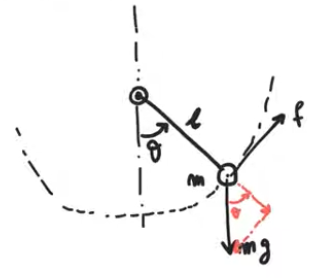
\includegraphics[width=\picwid]{pendolo.png}
 % pendolo.png: 316x278 px, 96dpi, 8.36x7.35 cm, bb=0 0 237 208
 %\label{Fig.:pendolo_semplice}
\end{figure}
Il sistema ha un punto di equilibrio?
Intuitivamente il punto di equilibrio è quello a $\theta=0$, in realtà anche
$\theta=\pi$ è un punto di equilibrio, in assenza della forza $f$ solo la forza
peso agisce sul sistema e in queste due posizioni è completamente bilanciata
dal vincolo dato che l'asta è rigida.

Se invece la forza $f$ applicata è diversa da zero e pari alla componente
tangente della forza peso $mg\sin(\theta)$ allora la condizione di equilibrio
si troverà in un punto diverso dai precedenti, inclinato di un certo angolo
$\theta$, e sarebbe in equilibrio anche nell'angolo $\pi - \theta$ rimanendo
fermo.

Il caso limite è quando l'asta diventa perfettamente orizzontale, il punto di
equilibrio diventa unico, $\theta = 90\text{\textdegree}$.

Se $f > mg$ il pendolo comincia a ruotare e non ci saranno più punti di
equilibrio.

Si riprende il modello analitico del pendolo ricavato in
\ref{eq.:pendolo_semplice}
$$
x_1 = \theta\ x_2 = \dot\theta\ u=f
$$
\begin{equation*}
\left\{\begin{aligned}
\dot x_1 &= \dot\theta = x_2 = f_1\\
\dot x_2 &= \ddot\theta = \frac{1}{mL} u - \frac{g}{L}  \sin(x_1) =f_2 \\
y &= \theta = x_1
\end{aligned}\right.
\end{equation*}

Il sistema ammette punti di equilibrio? Dalla definizione, se il sistema
ammette punti di equilibrio bisogna trovare una coppia
$(\overline{u},\overline{x})$ tali che la funzione di transizione $f$ sia pari
a zero.
$$
(\overline{u},\overline{x}) \Rightarrow f(\overline{u},\overline{x}) = 0
$$

Dunque si costruisce il sistema per ricavare lo stato di equilibrio
$$\left\{\begin{aligned}
&\overline{x}_2 = 0 \rightarrow \dot\theta = 0\\
&\frac{1}{m\cancel{L}} \overline{u} - \frac{g}{\cancel{L}}
\sin(\overline{x}_1)=0 \rightarrow \sin(\overline{x}_1) =
\frac{1}{mg}\overline{u}
\end{aligned}\right.$$
La velocità deve essere nulla e la soluzione è indipendente dalla lunghezza
dell'asta.

Analizzando la seconda equazione si ha che la funzione seno è limitata tra
$[-1,1]$ dunque
$$
\frac{|\overline{u}|}{mg} \leq 1 \Longleftrightarrow
|\overline{u}| \leq mg
$$

Le equazioni confermano quanto intuito precedentemente, la forza peso $mg$ deve
essere maggiore o uguale della forza $f$ applicata dall'esterno.

Si studiano i seguenti casi
$$|\overline{u}| \leq mg
\begin{aligned}
&\nearrow \\
& \\
&\\
&\searrow
\end{aligned}\
\begin{aligned}
&\\
&\\
&|\overline{u}|=mg \begin{aligned}
&\nearrow \\
&\searrow
\end{aligned}\ \begin{aligned}
&\overline{u} = mg \Rightarrow\sin(\overline{x}_1) = 1 \Rightarrow
\overline{x}_1 = \frac{\pi}{2}\\
&\\
&\overline{u} = -mg \Rightarrow \sin(\overline{x}_1) = -1 \Rightarrow
\overline{x}_1 = -\frac{\pi}{2}
\end{aligned}
&\\
&\\
&|\overline{u}|<mg \Rightarrow \overline{x}_1 = \begin{aligned}
&\nearrow \\
& \searrow
\end{aligned}\ \begin{aligned}
&\sin^{-1}\left(\frac{\pi}{mg}\right) \\
&\\
&\pi - \sin^{-1}\left(\frac{\pi}{mg}\right)
\end{aligned}
\\
&\\
\end{aligned}
$$
Si è quantificato numericamente il valore degli angoli di equilibrio del
sistema.


\section{Linearizzazione dei sistemi}
In mancanza della condizione di tempo invarianza può variare l'analisi del
sistema, verranno analizzati sistemi con discontinuità ma non sistemi che
variano con continuità nel tempo i loro parametri.

I sistemi non lineari sono composti da variabili e da parametri, i parametri
non sono mai forniti con un'accuratezza infinita, di conseguenza anche i
risultati in uscita avranno una certa incertezza.

Si suppone di modellare un sistema monodimensionale non lineare avendo fissato
una $\overline{u}(t)$ e si vuole mostrare l'andamento di $\dot x$ in funzione
di $x$, ricercando i vari punti di equilibrio.

%Curva di lavoro totale
\begin{figure}[h]
 \centering
 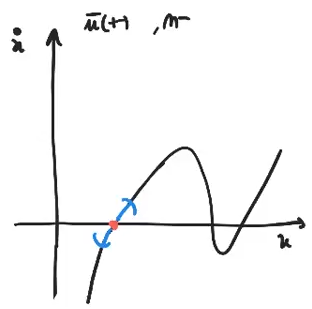
\includegraphics[width=\picwid]{curva_non_lineare.png}
 % curva_non_lineare.png: 312x309 px, 96dpi, 8.25x8.17 cm, bb=0 0 234 232
 \label{Fig.:curva_non_lineare}
\end{figure}

Si suppone che il sistema si trovi nel punto di lavoro $A$ indicato sul
grafico, nella realtà si troverà nell'intorno di quel punto oscillando in un
certo intervallo in funzione dei disturbi interni ed esterni al sistema.

Si suppone di ingrandire la curva nell'intorno del punto di lavoro

% Immagine ingrandita
\begin{figure}[h]
 \centering
 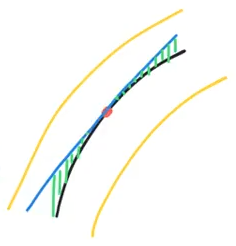
\includegraphics[width=\picwid]{curva_non_lineare_ingrandita.png}
 \label{Fig.:curva_non_lineare_ingrandita}
\end{figure}
Si considera una retta tangente alla curva nel punto di equilibrio, una retta è
sinonimo di un modello lineare, l'errore aggiuntivo commesso può ritenersi
trascurabile se minore dell'accuratezza fornita dal modello sesso.

Il vantaggio ottenuto da tale approssimazione è la possibilità di risolvere
analiticamente un sistema lineare piuttosto che cercare un teorema in grado di
risolvere quel particolare sistema non lineare.

Se si sposta di molto il punto di lavoro del sistema è necessario ricalcolare
la linearizzazione del sistema, non potendo più utilizzare la retta precedente.
Si ottiene ancora una buona approssimazione.

Ha senso linearizzare solo i punti di equilibrio, altrimenti il sistema non si
troverebbe nell'intorno di un punto, si potrebbe estendere il concetto anche a
punti di equilibrio dinamici.

$$\left\{
\begin{aligned}
\dot{x} &= f(x,u) \\
y &= g(x,u)
\end{aligned}\right.$$
Si ipotizza che le funzioni $f$ e $g$ siano sufficientemente regolari, ossia
che esista almeno il differenziale primo.

Si suppone inoltre che il sistema sottoposto ad un ingresso costante
$\overline{u}$ si trovi in un punto di equilibrio $\overline{x}$ a cui
corrisponde un'uscita di equilibrio $\overline{y}$, ossia
$$
(\overline{u},\overline{x},\overline{y}) \ \text{punto di equilibrio}
$$

Si applica la seguente posizione
$$
x(t) = \overline{x} + \delta x(t)
$$
dove $\delta x(t)$ è l'errore della traiettoria rispetto al punto di lavoro,
ovvero lo spessore definito prima nell'intorno del punto.

Analogamente per l'ingresso $u(t)$
$$
u(t) = \overline{u} + \delta u(t)
$$
Gli ingressi si suddividono in \textit{manipolabili} e \textit{non
manipolabili} dunque
anche gli ingressi sono affetti da errore e rumore,  è necessario tenere conto
di questi errori mediante
$$
y(t) = \overline{y}+\delta y(t)
$$

Tutte le precedenti equazioni sono vettoriali.

Derivando l'equazione dello stato
$$
\dot{x} = \dot{\overline{x}} + \dot{\delta x} = \dot{\delta x}
$$
quindi la variazione dello stato coincide con la variazione locale. Si può
sviluppare in serie di Taylor nel punto di equilibrio
\begin{equation}
\dot{\delta x} = \cancel{f(\overline{x},\overline{u})} + \left.\frac{\partial
f}{\partial x}\right|_{\text{eq}}\delta x + \left.\frac{\partial f}{\partial
u}\right|_{\text{eq}}\delta u + o(\delta x, \delta u)
\label{eq.:linearizzazione_sistema}
\end{equation}
La funzione di transizione valutata su un punto di equilibrio è nulla per
definizione di punto di equilibrio, il termine $\frac{\partial f}{\partial x}$
è una matrice Jacobiana con numero di righe pari al numero di righe della $f$
dunque $n$ ed un numero di colonne pari al numero di elementi della $x$, ancora
$n$ quindi è una matrice $n\times n$, la matrice verrà chiamata $A$.

Il termine $\frac{\partial f}{\partial u}$ ha invece $n$ righe ed $m$ colonne
dove $m$ è il numero di ingressi, verrà chiamata $B$.

Si riscrive la \ref{eq.:linearizzazione_sistema} trascurando l'o-piccolo si
ottiene

$$\begin{aligned}
\dot x &= \dot{\delta x} = A\delta x + B \delta u
\end{aligned}$$
quella ottenuta è proprio l'equazione di un sistema dinamico lineare con
variabile di stato pari a $\delta x$ ed ingresso pari a $\delta u$

La variazione dell'uscita invece sarà
$$\begin{aligned}
y &= \overline{y} + \delta y = g(\overline{x},\overline{u}) +
\left.\frac{\partial
g}{\partial x}\right|_{\text{eq}}\delta x + \left.\frac{\partial g}{\partial
u}\right|_{\text{eq}}\delta u + o(\delta x, \delta u) \\
\delta g &\simeq C\delta x + D \delta u
\end{aligned}$$
Anche la variazione dell'uscita è lineare con la variazione dello stato e
dell'ingresso.

Dopo aver risolto il sistema delle variazioni si somma con il sistema dei
punti di equilibrio e si ottiene la risoluzione dell'intero sistema.

In molti casi la coppia $(0,0)$ è un punto di equilibrio, in questo specifico
caso è sufficiente calcolare solo le variazioni, dato che andrebbero poi
sommate con un valore nullo di ingresso ed equilibrio.

Si riprende l'esempio analizzato alla sezione \ref{sec.:equilibrio_del_pendolo}
$$\left\{\begin{aligned}
\dot x_1 &= x_2\\
\dot x_2 &= - \frac{g}{l}\sin{x_1} + \frac{1}{mL}u \\
y &= x_1
\end{aligned}\right.$$

Va dunque calcolata la matrice $A$
$$ A =
\left.\frac{\partial f }{\partial x}\right|_{\text{eq}} = \begin{pmatrix}
 \left.\frac{\partial f_1}{\partial x_1}\right|_{\text{eq}}
 & \left.\frac{\partial f_1}{\partial x_2}\right|_{\text{eq}} \\
 \left.\frac{\partial f_2}{\partial x_1}\right|_{\text{eq}}
 & \left.\frac{\partial f_2}{\partial x_2}\right|_{\text{eq}}
\end{pmatrix} =
\begin{pmatrix}
 0 & 1\\
 -\frac{g}{L}\cos(\overline{x}_1) & 0
\end{pmatrix} $$

Si ripete il procedimento rispetto all'ingresso e si calcola la matrice $B$
$$
B = \left.\frac{\partial f }{\partial u}\right|_{\text{eq}} =
\begin{pmatrix}
 \left.\frac{\partial f_1}{\partial u}\right|_{\text{eq}} \\
 \left.\frac{\partial f_2}{\partial u}\right|_{\text{eq}}
\end{pmatrix} =
\begin{pmatrix}
0 \\
\frac{1}{mL}
\end{pmatrix}
$$
La seconda matrice è costante e non dipende dai punti di equilibrio.

Si esegue la stessa operazione per l'equazione delle uscite
$$
C = \left.\frac{\partial g}{\partial x}\right|_{\text{eq}} =
\begin{pmatrix}
 \left.\frac{\partial g}{\partial x_1}\right|_{\text{eq}}  &
 \left.\frac{\partial g}{\partial x_2}\right|_{\text{eq}}
\end{pmatrix} =
\begin{pmatrix}
 1 & 0
\end{pmatrix}
$$

Infine dato che il sistema è strettamente proprio non è necessario calcolare la
matrice $D$ dato che sarà sicuramente nulla, se ne riporta in ogni caso la
definizione
$$
D = \left.\frac{\partial g}{\partial u}\right|_{\text{eq}} =
0
$$
L'unica matrice che varia al variare del punto di equilibrio è la prima.

Si calcolano le matrici $A'$ ed $A''$ nei due punti di equilibrio
$$
\overline{u} = 0 \left\langle
\begin{aligned}
 \\
 \overline{x'} &= \begin{pmatrix}
                  0 \\ 0
                 \end{pmatrix} \Rightarrow
                 A' = \left.\frac{\partial f}{\partial x}
                            \right|_{\begin{aligned}
                                      x &= \overline{x'}\\
                                      u &= 0
                                     \end{aligned}} =
                                     \begin{pmatrix}
                                      0 & 1 \\
                                      -\frac{g}{L} & 0
                                     \end{pmatrix}
\\
 \overline{x''} &= \begin{pmatrix}
                   \pi \\ 0
                  \end{pmatrix} \Rightarrow
                 A'' = \left.\frac{\partial f}{\partial x}
                            \right|_{\begin{aligned}
                                      x &= \overline{x'}\\
                                      u &= 0
                                     \end{aligned}} =
                                     \begin{pmatrix}
                                      0 & 1 \\
                                      \frac{g}{L} & 0
                                     \end{pmatrix}
\end{aligned} \right.
$$



\subsection{Diagonalizzazione per similitudine}
Sia un'applicazione $A\in\mathbb{R}^{n\times n}$ di semplice struttura, ovvero
con $n$ autovalori distinti e di conseguenza $n$ autovettori distinti e
indipendenti tra loro, in uno spazio di $n$ dimensioni, dunque forniscono una
base.
$$
\left\{\begin{aligned}
\lambda_1& \rightarrow u_1\\
\vdots& \quad\ \  \vdots \\
\lambda_n & \rightarrow u_n
\end{aligned}\right.
$$
Si pongono i vettori per colonna in una matrice quadrata $U$
$$
U = [u_1, \ldots, u_n]
$$
Il rango della matrice sarà certamente $n$, composta da $n$ vettori linearmente
indipendenti, sarà una matrice non singolare.
La matrice $U$ può essere usata per realizzare una trasformazione di
similitudine.
$$
x = U\tilde{x}
$$
La matrice $U$ prende il nome di \textit{matrice modale},
la matrice della dinamica del sistema si può riscrivere come
$$
\tilde{A} = U^{-1}AU
$$
con $\tilde{A}$ la matrice di similitudine dello stesso sistema in una base
differente, \textit{equivalente} alla matrice $A$ di partenza.

Sviluppando i prodotti
$$
\tilde{A} = U^{-1}AU = \begin{bmatrix}
                        \lambda_1 & 0 & 0 \\
                        0 & \ddots & 0 \\
                        0 & 0 & \lambda_n
                        \end{bmatrix} = \Lambda
$$
La matrice $\Lambda$ viene denominata \textit{matrice degli autovalori}.
Si è ottenuta una matrice della dinamica del sistema di tipo diagonale, con
solo gli autovalori sulla diagonale.
La trasformazione di similitudine non altera gli autovalori del sistema.

Questa rappresentazione prende il nome di \textit{diagonalizzazione per
similitudine}, si è diagonalizzata la matrice della dinamica.

Si vuole dimostrare la precedente
$$\begin{aligned}
U^{-1} A[u_1 \ldots u_n] &= U^{-1} [Au_1, Au_2, \ldots, Au_n] =
U^{-1}[\lambda_1u_1,\lambda_2u_2,\ldots,\lambda_nu_n] =\\
&=U^{-1} [u_1,u_2,\ldots,u_n] \begin{bmatrix}
                        \lambda_1 & 0 & 0 \\
                        0 & \ddots & 0 \\
                        0 & 0 & \lambda_n
                             \end{bmatrix} = I\Lambda = \Lambda
\end{aligned}$$

\chapter{Analisi dei sistemi LTI nel dominio del tempo}
La forma ISU dei sistemi di questo tipo è
$$\left\{\begin{aligned}
\dot x &= Ax +Bu \\
y &= Cx + Du
\end{aligned}\right.$$
Le matrici caratteristiche sono costanti, ma il legame rispetto allo stato è
implicito, per ricavare esplicitamente il legame tra uscita e stato è necessario
integrare il sistema.

\section{Risoluzione analitica di un sistema differenziale}
Per risolvere il sistema è necessario determinare l'integrale generale, dato
dalla somma dell'integrale dell'omogenea associata
nominata $x_h(t)$ e di una qualunque soluzione particolare $x_p(t)$
$$
x(t) =x_h(t) + x_p(t)
$$
Soluzione omogenea $\dot x_h = Ax_h$, si suppone che la soluzione sia del tipo
$$
e^{\lambda t}\cdot c\quad \lambda \in \mathbb{R}, c\in \mathbb{R}^n
$$

Sostituendo l'ipotesi di soluzione nel sistema e differenziando si ottiene
$$
\lambda \cancel{e^{\lambda t}} c = A\cancel{e^{\lambda t}} c
$$
$$
\lambda c = A c \Leftrightarrow (\lambda I -A)c = 0
$$
Questa equazione è vera solo se $\lambda$ è un autovalore (con $c\neq
\underline{0}$).
Esistono solo $n$ soluzioni possibili (nell'ipotesi che la matrice $A$ sia di
semplice struttura, non è un'ipotesi necessaria).

Qualunque soluzione $x_h$ combinazione lineare delle soluzioni precedentemente
ricavata, è ancora soluzione del sistema.
$$
x_h(t) = \sum_{i=1}^n e^{\lambda_i t} c_i
$$
Analogamente si potrebbe procedere con la soluzione particolare.

\subsection{Matrice esponenziale}
Si indica simbolicamente con
\begin{equation}
e^{At} \stackrel{\text{def}}{=} \sum_{k=0}^{+\infty} \frac{A^k t^k}{k!}
\end{equation}
È una serie nel tempo e non una matrice di esponenziali.

Si cercano le ipotesi di convergenza della serie, la sua norma è maggiorata da
una serie assolutamente convergente (per ciascun valore di $t$)
$$
\left|\left|e^{At}\right|\right| = \left|\left|\sum_{k} \frac{A^k
t^k}{k!}\right|\right| \leq \sum_k \frac{\left|\left|A^k\right|\right| t^k}{k!}
\leq \sum_k \frac{a^kt^k}{k!} \stackrel{\text{def}}{=}e^{at}
$$
La norma della somma è minore o uguale alla somma delle norme e i tempi sono
assunti positivi.
Si ricava il coefficiente $a^k$ dato che $||A^k|| \leq ||A||^k = a^k $, quella
ottenuta è la definizione di esponenziale scalare.

Si vuole scrivere una soluzione analitica della matrice esponenziale, si
supponga che sia diagonalizzabile per similitudine, ossia se ne possa costruire
la matrice modale, ciò è sicuramente vero se la matrice è di semplice struttura.
In generale è sufficiente che per ogni autovalore la molteplicità
algebrica coincida con quella geometrica, ossia siano presenti $n$ autovettori
distinti (esista una base).
Si può costruire la matrice $\Lambda$ degli autovalori
$$
\Lambda = U^{-1}AU \Leftrightarrow A=U\Lambda U^{-1}
$$
Si eleva la matrice $A$ a potenza
$$
A^k = (U\Lambda U^{-1})^k = U\Lambda U^{-1} \cdot U\Lambda U^{-1} \cdot
\ldots\cdot U\Lambda U^{-1}\ k\ \text{volte}
$$
Si nota che sono sempre presenti $k$ prodotti $U^{-1}U$ pari alla matrice
identità, dunque
$$
A^k = U\Lambda^kU^{-1}
$$
Ma lambda è una matrice diagonale, moltiplicata per sé stessa fornisce ancora
una matrice diagonale
\begin{equation}
A^k = U \begin{bmatrix}
        \lambda_1^k & 0 & 0      \\
        \vdots & \ddots & \vdots \\
        0 & 0 & \lambda_n^k
        \end{bmatrix} U^{-1} =
\begin{bmatrix}u_1 & \ldots & u_n\end{bmatrix} \begin{bmatrix}
        \lambda_1^k & 0 & 0      \\
        \vdots & \ddots & \vdots \\
        0 & 0 & \lambda_n^k
        \end{bmatrix}
        \begin{bmatrix}
        v_1^T\\ \vdots \\ v_n^T
        \end{bmatrix}
\label{eq.:matrice_esponenziale}
\end{equation}
Sviluppando i prodotti
\begin{equation}
A^k = \sum_{i=1}^n \lambda_i^k u_i v_i^T
\label{eq.:forma_spettrale}
\end{equation}
Si ottiene la somma di $n$ matrici $n\times n$ denominate residui
polari $R_i$ moltiplicate per $\lambda^k$.
Una proprietà dei residui polari, nel caso di matrice diagonalizzabile, è che
hanno rango pari ad uno.

La \ref{eq.:forma_spettrale} prende il nome di \textit{forma spettrale} (o
forma \textit{diadica}) della matrice potenza.

\subsubsection{Calcolo della matrice esponenziale}
Si supponga che $A$ sia diagonalizzabile, si vuole calcolare la matrice
esponenziale
$$\begin{aligned}
e^{At} &\stackrel{\text{def}}{=} \sum_{k=0}^{+\infty} \frac{A^kt^k}{k!}=
\sum_{k=0}^{+\infty} \frac{U\Lambda^kU^{-1}t^k}{k!} =
U\left(\sum_{k=0}^{+\infty}\frac{\Lambda^kt^k}{k!}\right)U^{-1}= \\
       &= U\begin{bmatrix}
            \sum_{k=0}^{+\infty} \frac{\lambda_1^kt^k}{k!} & 0 & 0 \\
            0 & \ddots & 0 \\
            0 & 0 & \sum_{k=0}^{+\infty}\frac{\lambda_n^kt^k}{k!}
            \end{bmatrix}U^{-1} = U\begin{bmatrix}
                                    e^{\lambda_1t} & 0 & 0 \\
                                    0 & \ddots & 0 \\
                                    0 & 0 & e^{\lambda_n t}
                                    \end{bmatrix}U^{-1} = \\
        &= \sum_{i=1}^n e^{\lambda_i t} u_i v_i^T
\end{aligned}$$

Anche la matrice esponenziale può essere calcolata mediante la sua forma
diadica o spettrale.
Riassumendo:
\begin{enumerate}
 \item Calcolo $\lambda_i, u_i\ i=1,\ldots,n$
 \item Verificare che $A$ sia diagonalizzabile, $m_{ai} = m_{gi} \ \forall i$
 \item (Se 2 vera) Costruzione della matrice modale $U$ e calcolo della sua
 inversa $U^{-1}\ \ (v_i^T)$
 \item Costruzione della matrice esponenziale della matrice degli autovalori
$e^{\Lambda t}$
 \item Calcolo di $e^{A t} =  U e^{\Lambda t} U^{-1}$ oppure mediante la
 sommatoria della forma spettrale.
\end{enumerate}

\newpage
\subsubsection{Esempio numerico}
Sia la matrice
$$
A = \begin{bmatrix}
    0 & 1 \\
    -2 & -3
    \end{bmatrix}
$$
\begin{enumerate}
\item Calcolo autovalori e autovettori

$p(\lambda) = |\lambda I -A| =
\text{det}\begin{pmatrix}
                                                \lambda & -1 \\
                                                2 & \lambda +3
                                                \end{pmatrix} =
\lambda(\lambda+3)+2 = \lambda^2 + 3\lambda +2 = 0$

Le soluzioni
$$
\begin{aligned}
\lambda_1 &= -1 \\
\lambda_2 &= -2
\end{aligned}
$$
Calcolo degli autovettori
$$
(\lambda_1 I -A)u_1 = \begin{pmatrix}
                        -1 & -1 \\
                        2 & 2
                        \end{pmatrix} \begin{pmatrix}
                                      u_{11} \\ u_{12}
                                      \end{pmatrix} = \begin{pmatrix}
                                      0 \\ 0
                                      \end{pmatrix}
$$
La matrice $ (\lambda_1 I -A)u_1$ è per costruzione singolare dato che
$\lambda$ è un autovalore, perde di rango una volta (dato che è di semplice
struttura e gli autovalori hanno molteplicità uno).
Per questo motivo è sufficiente risolvere una sola equazione e gli autovettori
saranno proporzionali tra di loro, si può assegnare arbitrariamente una
componente dell'autovettore (ad esempio $u_{12}=1$)
$$
- u_{11} - u_{12} = 0 \Rightarrow u_{11} = -1 \Rightarrow u_1 = \begin{pmatrix}
-1 \\ 1
\end{pmatrix}
$$

Può essere comodo normalizzare gli autovettori normalizzati ma non è necessario
in questo corso.

Secondo autovettore:
$$
(\lambda_2 I -A)u_1 = \begin{pmatrix}
                        -2 & -1 \\
                        2 & 1
                        \end{pmatrix} \begin{pmatrix}
                                      u_{21} \\ u_{22}
                                      \end{pmatrix} = \begin{pmatrix}
                                      0 \\ 0
                                      \end{pmatrix}
$$
Assegnando arbitrariamente $u_{21} = 1$
$$
-2u_{21} - u_{22} = 0 \Rightarrow  u_{22} = -2 \Rightarrow u_2 = \begin{pmatrix}
1 \\ -2
\end{pmatrix}
$$

\item Verifica diagonalizzabilità, passaggio scontato dato che la matrice è di
semplice struttura.

\item Costruzione della matrice modale
$$
U = \begin{bmatrix}u_1 & u_2\end{bmatrix} = \begin{bmatrix}
                                            -1 & 1 \\
                                            1 & -2
                                            \end{bmatrix} \qquad U^{-1} =
\begin{bmatrix}
-2 & -1 \\
-1 & -1
\end{bmatrix}\begin{matrix}
\rightarrow & v_1^T \\ \rightarrow & v_2^T
\end{matrix}
$$

\item Costruzione della matrice esponenziale degli autovalori $e^{\Lambda t}$
$$
e^{\Lambda t} = \begin{bmatrix}
                e^{-t} & 0 \\
                0 & e^{-2 t}
                \end{bmatrix}
$$

\item Costruzione della matrice esponenziale $e^{At}$ attraverso la
decomposizione spettrale
$$\begin{aligned}
e^{At} &= Ue^{\Lambda t} U^{-1} = \begin{pmatrix}
                                    -1 & 1 \\
                                    -1 & -2
                                    \end{pmatrix} \begin{pmatrix}
                                                e^{-t} & 0 \\
                                                0 & e^{-2t}
                                                \end{pmatrix} \begin{pmatrix}
                                                -2 & -1 \\
                                                -1 & -1
                                                \end{pmatrix} = \\
    &= \begin{pmatrix}
        -e^{-t} & e^{-2t} \\
        -e^{-t} & -2e^{-2t}
        \end{pmatrix}\begin{pmatrix}
                    -2 & -1 \\
                    -1 & -1
                    \end{pmatrix} = \begin{pmatrix}
                                    2e^{-t}-e^{-2t} & e^{-t}-e^{-2t}\\
                                    2e^{-t}+2e^{-2t} & e^{-t}+e^{-2t}
                                    \end{pmatrix}
\end{aligned}$$
La matrice esponenziale è al più combinazione lineare delle funzioni del tempo
presenti nella matrice ricavata al punto 4 chiamate anche \textbf{modi
naturali} del sistema, potrebbe contenerne di meno.
\end{enumerate}

\subsubsection{Complementi}
Sia la matrice $A\in\mathbb{R}^{n\times n}$ ed un suo autovalore $\lambda_i$ a
cui è associato l'autovettore $u_i$
$$
A\in\mathbb{R}^{n\times n}\ \lambda_i\ u_i
\stackrel{\text{def}}{\Leftrightarrow} Au_i = \lambda_iu_i
$$
Si vuole dimostrare che se si considera la matrice potenza $A^k$
$$
A^k : A^ku_i = \lambda_i^ku_i
$$
La matrice $A^k$ è quadrata, potrebbe essere chiamata $B$, se moltiplicata per
un vettore si ottiene lo stesso vettore moltiplicato per uno scalare, si
ottiene cioè la definizione di autospazio invariante monodimensionale.
La matrice potenza $A^k$ ha come autovettori gli stessi autovettori della
matrice $A$, l'elevazione a potenza non cambia gli autovettori, gli autovalori
invece sono le potenze degli autovalori di partenza.
1:29:14

\subsection{Teorema di Caley-Hamilton}
Si consideri una matrice $A$ quadrata
$$
A\in\mathbb{R}^{n\times n},\ p(\lambda) = \text{det}(\lambda I-A) = \lambda^n +
\alpha_{n-1}\lambda^{n-1} + \ldots + \alpha_0 \lambda^0
$$
Ogni matrice quadrata è soluzione del proprio polinomio caratteristico, con
abuso di notazione
$$
p(A) = A^n + \alpha_{n-1}A^{n-1}+ \ldots + \alpha_0 A^0 =
\underline{\underline{0}}
$$
con $A^0 = I$ e $p(A)$ un polinomio di matrici.

Si dimostra il teorema con l'ipotesi semplificativa ma non necessaria di
matrice A di semplice struttura
$$
p(A)\cdot u_i = A^nu_i + \alpha_{n-1}A^{n-1}u_i + \ldots + \alpha_0 u_i =
(\lambda_i^n+\alpha_{n-1}\lambda_i^{n-1}+\ldots + \alpha_0)u_i = \underline{0}\
\forall i
$$
Quello ottenuto all'ultimo termine è proprio il polinomio caratteristico che
valutato nell'autovalore è nullo per definizione.

Nell'ipotesi di semplice struttura i diversi autovettori $u_i$ formano una
base, di conseguenza tutti gli altri vettori saranno combinazione lineare degli
autovettori e restituiranno anch'essi il vettore nullo nulli se moltiplicati
per il polinomio di matrici $p(A)$
$$
p(A) = 0 \Rightarrow p(A)\cdot x = \underline{0} \ \ \forall x\in X^n
$$
La matrice deve necessariamente avere rango nullo perché moltiplicata per un
vettore dia come risultato un vettore nullo, di conseguenza, l'unica matrice di
rango nullo è la matrice nulla
$$
\rho(p(A))=0 \Rightarrow p(A) = \underline{\underline{0}}
$$

Si può isolare il termine $A^n$ dal polinomio di matrici, $k\geq 0$
$$
A^n = \sum_{i=0}^{n-1}(-\alpha_i)A^i \Rightarrow A^{n+k} =
\sum_{i=0}^{n-1}\beta_iA^i
$$
La potenza di ordine $n$ è una combinazione lineare di potenze fino all'ordine
$n-1$, si dimostra per induzione, vera per $k=0$, si ipotizza vera per un
generico $k$, si dimostra che è vera per $k+1$, si ottiene la dimostrazione del
teorema.

\subsection{Tecnica del polinomio interpolante - Matrice di Vandermonde}
Si vuole calcolare ancora la matrice esponenziale $e^{At}$
\begin{equation}
e^{At} \stackrel{\text{def}}{=} \sum_{k=0}^{+\infty} \frac{A^kt^k}{k!} =
\sum_{i=0}^{n-1} \alpha_i(t)A^i
\label{eq.:esponenziale_polinomio_interpolante}
\end{equation}
Sfruttando quanto ricavato dal teorema di Caley-Hamilton si potrebbe riscrivere
la potenza come una combinazione lineare di potenze di ordine inferiore.
I coefficienti $\alpha_i(t)$ raggruppano tutti i coefficienti della potenza
$i$-esima della matrice $A$, è presente la dipendenza del tempo a causa dei
termini $t^k$.
Se si potessero calcolare i coefficienti $\alpha_i(t)$ si potrebbe ridurre la
serie ad una somma finita di matrici.

$$
e^{At} \cdot u_1 = \sum_{i=0}^{n-1} \alpha_i(t)A^iu_1 =
\sum_{i=0}^{n-1}\alpha_i(t)\lambda^i_1 u_1 = e^{\lambda_1 t} u_1
$$
Si può ripetere questo passaggio per tutti gli autovettori della matrice $A$
$$
e^{At}u_n = \sum_{i=0}^{n-1} \alpha_i(t)A^iu_n = \sum_{i=0}^{n-1}
\alpha_i(t)\lambda_n^i u_n = e^{\lambda_n t} u_n
$$
Essendo gli autovettori non nulli allora
$$
\sum_{i=0}^{n-1} \alpha_i(t) \lambda^i_n = e^{\lambda_n t}
$$
Riscrivendo il sistema in forma compatta
$$
\begin{bmatrix}
1 &\lambda_1 & \lambda_1^2 & \ldots & \lambda_1^{n-1}\\
\vdots &\vdots  &\vdots    &              & \vdots&         \\
1  &\lambda_n & \lambda_n^2 & \ldots &\lambda_n^{n-1}
\end{bmatrix}
\begin{bmatrix}
                \alpha_0(t) \\ \vdots \\ \alpha_{n-1}(t)
                \end{bmatrix} = \begin{bmatrix}
                                e^{\lambda_1 t} \\ \vdots \\ e^{\lambda_n t}
                                \end{bmatrix}
$$
La prima matrice prende il nome di \textbf{matrice di Vandermonde}, si indica
con \linebreak $V(\lambda_1,\ldots,\lambda_n)$, funzione di $n$ elementi.

Il determinante della matrice di Van der Monde è pari alla produttoria delle
differenze di tutti i coefficienti
$$
\text{det}\left(V\left(\lambda_1,\ldots,\lambda_n\right)\right) = \prod_{1\leq
i < j \leq n } (\lambda_j - \lambda_i)
$$
L'unico caso che può annullare la produttoria è quando due coefficienti con
indice diverso siano uguali, ovvero $A$ non sia di semplice struttura, in caso
contrario, invertendo la matrice si possono ricavare i coefficienti
$$
\begin{bmatrix}
\alpha_0(t)\\
\vdots \\
\alpha_{n-1}(t)
\end{bmatrix} =
V^{-1}(\lambda_1,\ldots,\lambda_n)
\begin{bmatrix}
e^{\lambda_1 t}\\
\vdots \\
e^{\lambda_n t}
\end{bmatrix}
$$
Sostituiti nell'equazione \ref{eq.:esponenziale_polinomio_interpolante}, dopo
aver calcolato le potenze della matrice $A$ permettono di calcolare la matrice
esponenziale con la somma di finiti termini.

Rispetto al metodo precedente non è necessario calcolare gli autovettori ma
\textbf{è necessario che la matrice $A$ sia di semplice struttura}.

\subsubsection{Procedura operativa}
\begin{enumerate}
 \item Calcolo degli autovalori
 \item Verifica che i $\lambda_i$ siano distinti, ossia che $A$ sia semplice
 \item Se si la 2. risoluzione del sistema
$V(\lambda_1,\ldots,\lambda_n)\begin{bmatrix}
\alpha_0(t) \\ \vdots \\ \alpha_{n-1}(t) \end{bmatrix}= \begin{bmatrix}
e^{\lambda_1 t } \\ \vdots \\ e^{\lambda_n t}
\end{bmatrix}$
\item Calcolo della matrice esponenziale $e^{At} = \sum_{i=0}^{n-1}
\alpha_i(t)A^i$
\end{enumerate}

\subsubsection{Esempio numerico}
Si riprende la stessa matrice utilizzata nel metodo della diagonalizzazione
(vedi paragrafo \ref{sec.:metodo_diagonalizzazione})
$$
A = \begin{bmatrix}
0 & 1\\
-2 & -3
\end{bmatrix}
$$
\begin{enumerate}
\item $p(\lambda) = \text{det} (\lambda I -A) = 0\Rightarrow \lambda_1 = -1,\
\lambda_2 = -2$
\item $\lambda_1\neq \lambda_2 \Rightarrow A $ semplice struttura
\item Costruzione e risoluzione del sistema $V\alpha_n(t) = e^{\lambda_n t}$
$$
\begin{bmatrix}
1 & -1 \\
1 & -2
\end{bmatrix}\begin{bmatrix}
\alpha_0(t) \\ \alpha_1 (t)
\end{bmatrix} =
\begin{bmatrix}
e^{-t} \\
e^{-2t}
\end{bmatrix}\Rightarrow \begin{bmatrix}
\alpha_0(t) \\ \alpha_1 (t)
\end{bmatrix} = - \begin{bmatrix}
-2 & 1 \\
-1 & 1
\end{bmatrix}\begin{bmatrix}
e^{-t} \\ e^{-2t}
\end{bmatrix}
$$
Sviluppando si ottiene
$$\left\{\begin{aligned}
\alpha_0(t) &= 2e^{-t} - e^{-2t}\\
\alpha_1(t) &= e^{-t} -e^{-2t}
\end{aligned}\right.$$
\item Calcolo della matrice esponenziale
$$\begin{aligned}
e^{At} &= \alpha_0(t)I + \alpha_1(t) A^1 =\\
&=\begin{pmatrix}
2e^{-t}-e^{-2t} & 0 \\
0 & 2e^{-t}-e^{-2t}
\end{pmatrix} + \begin{pmatrix}
0 & e^{-t}-e^{-2t} \\
-2e^{-t}+2e^{-2t} & -3e^{-t} + 3e^{-2t}
\end{pmatrix} =\\
&= \begin{pmatrix}
2e^{-t}-e^{-2t} & e^{-t}-e^{-2t}\\
-2e^{-t} + e^{-2t} & -e^{-t}+2e^{2t}
\end{pmatrix}
\end{aligned}$$
\end{enumerate}

\newpage
\subsubsection{Riassunto dei due metodi precedenti}
Sia $A$ una matrice di semplice struttura, si può calcolare la matrice
esponenziale mediante due metodi
\begin{enumerate}
 \item Diagonalizzazione

 Per $n$ autovalori distinti
 $$
 \exists\ n \text{ autovettori indipendenti } u_i \Rightarrow U=[u_1,\ldots,u_n]
 $$
 $$\begin{aligned}
 A &= U\Lambda U^{-1} = \sum_{i=1}^{n} \lambda_i u_iv_i^T\\
 e^{At} &= Ue^{\Lambda t} U^{-1} = \sum_{i=1}^{n} e^{\lambda_i}u_iv_i^T
 \end{aligned}$$
 Ricordando che il prodotto tra autovettori e le colonne della matrice modale
inversa si ottengono le matrici $R_i$ denominate \textit{matrici dei residui
polari}, avranno rango unitario in questo caso, hanno in generale il rango pari
alla molteplicità geometrica dell'autovettore $i-$esimo $u_i$.
$$
u_i v_i^T = R_i
$$

\item Polinomio interpolante

Si costruisce la matrice di Vandermonde, si calcola il vettore dei coefficienti
$\alpha$ e si calcola la matrice esponenziale
$$
V(\lambda_1,\ldots,\lambda_n) \Rightarrow \alpha_i(t):
\begin{bmatrix}
\alpha_0(t) \\
\vdots \\
\alpha_{n-1}(t)
\end{bmatrix} = V^{-1}(\lambda_1,\ldots,\lambda_n)
\begin{bmatrix}
e^{\lambda_1t}\\
\vdots \\
e^{\lambda_nt}
\end{bmatrix}
$$
$$
e^{At} =\sum_{i=0}^{n-1} \alpha_i(t)A^i
$$
\end{enumerate}

\subsection{Matrice non semplice}
Si suppone che la matrice non sia di semplice struttura ma solo
diagonalizzabile, esisteranno $m$ autovalori distinti $(m < n)$, dunque il
generico autovalore $\lambda_i$ avrà molteplicità algebrica maggiore di uno.
Per calcolare gli autovettori si risolvono i sistemi
$$
(A-\lambda_iI)u_i=0
$$
la molteplicità geometrica del generico autovettore è
$$
m_{gi}= n-\rho(A-\lambda_iI)
$$
Se la molteplicità geometrica è inferiore di quella algebrica, si troveranno
meno autovettori di quanti sono necessari a diagonalizzare la matrice che
risulterà dunque \textbf{non diagonalizzabile}. $1< m_{gi} \leq  m_{ai} \leq n $

Considerato il generico autovalore $\lambda_i$ si pongono i corrispondenti
autovettori in colonna
$$
\lambda_i \rightarrow U_i=[u_{i_1},\ldots,u_{i_{m_{ai}}}]
$$
Si costruisce in seguito la matrice modale affiancando i blocchi appena ottenuti
$$
U = [U_1,U_2,\ldots,U_m]
$$
Di conseguenza si costruisce una matrice degli autovalori dove ogni autovalore
è ripetuto sulla diagonale per un numero di volte pari alla sua molteplicità
(algebrica o geometrica, coincidono)
$$
A=U
\begin{bmatrix}
\lambda_1 &0 &0 &0 &0 &0 &0 &0 &0 &0 \\
0    &\ddots &0 &0 &0 &0 &0 &0 &0 &0 \\
0 &0 &\lambda_1 &0 &0 &0 &0 &0 &0 &0 \\
0 &0 &0 &\lambda_2 &0 &0 &0 &0 &0 &0 \\
0 &0 &0 &0    &\ddots &0 &0 &0 &0 &0 \\
0 &0 &0 &0 &0 &\lambda_2 &0 &0 &0 &0 \\
0 &0 &0 &0 &0 &0    &\ddots &0 &0 &0 \\
0 &0 &0 &0 &0 &0 &0 &\lambda_n &0 &0 \\
0 &0 &0 &0 &0 &0 &0 &0    &\ddots &0 \\
0 &0 &0 &0 &0 &0 &0 &0 &0 &\lambda_n
\end{bmatrix}U^{-1}
$$
Raccogliendo i termini
$$
A = \sum_{i=1}^m \lambda_i \cdot \sum_{j=1}^{m_{ai}} u_{ij}\cdot v_{ij}^T
$$
Sono necessari due pedici in quanto il primo indica il gruppo di autovettori
associati all'autovalore $i$ mentre il secondo è associato alla molteplicità
$m_{ai}$ e permette di moltiplicare l'autovalore per ogni suo autovettore.

Analogamente per la matrice esponenziale
$$
e^{At} = \sum_{i=1}^m e^{\lambda_i t} \cdot \sum_{j=1}^{m_{ai}} u_{ij}\cdot
v_{ij}^T
$$
Con un abuso di notazione si potrebbero indicare autovalori uguali con nomi
diversi, in modo da avere comunque un numero di autovalori pari al numero di
autovettori e riprendere la notazione del caso precedente con matrice semplice.

I vettori  $u_i$ vengono chiamati autovettori \textit{destri} ovvero devono
moltiplicare a destra la matrice $A$ per restituire l'autovalore.

Gli autovettori $v_i$ vengono invece chiamati autovettori sinistri (presi
sempre per colonna)
$$\begin{aligned}
u_i &: Au_i = \lambda_i u_i\\
v_i &: v_iA = \lambda_i v_i
\end{aligned}$$

\subsection{Autovalori complessi e coniugati}
Ad ogni coppia di autovalori complessi e coniugati corrisponderà una coppia di
autovettori complessi e coniugati, il resto della notazione non cambia, si
risolveranno due sistemi di equazioni, uno per la parte reale ed uno per la
parte immaginaria.

Si introduce una variante della diagonalizzazione, chiamata \textbf{forma
reale} della matrice degli autovalori.
Per avere tutti termini reali sulla matrice degli autovalori sarà necessario
perdere l'ipotesi di matrice diagonale ma di avere invece una matrice diagonale
a blocchi.

Si considera per semplicità di analisi un caso di $n=3$ ed un autovalore reale
ed uno complesso e coniugato, in caso contrario si ripete il risultato ottenuto.

I tre autovalori saranno
$$\left\{\begin{matrix}
\lambda \\ \alpha+j\omega \\ \alpha-j\omega
\end{matrix}\right.$$
Si devono costruire gli autovettori complessi e coniugati
$$\left\{\begin{aligned}
&(A-(\alpha+j\omega)I)(u_a+ju_b) = \underline{0} + j\underline{0}\\
&(A-(\alpha-j\omega)I)(u_a-ju_b) = \underline{0} + j\underline{0}
\end{aligned}\right.$$
Si sviluppa la prima riga
$$\begin{aligned}
&(A-(\alpha+j\omega))(u_a + ju_b) = \underline{0} +
j\underline{0}\Rightarrow
\left\{\begin{aligned}
&Au_a - \alpha u_a + \omega u_b = 0\\
&Au_b - \omega u_a -\alpha u_b = 0
\end{aligned}\right.
\end{aligned}$$
Si porta a sinistra la matrice $A$ e si lasciano gli altri termini a destra
$$
\left\{\begin{aligned}
Au_a &= \alpha u_a - \omega u_b \\
Au_b &= \omega u_a + \alpha u_b
\end{aligned}\right. \Leftrightarrow A (u_a \ u_b) = (u_a \ u_b)
\begin{pmatrix}
\alpha & \omega\\
-\omega & \alpha
\end{pmatrix}
$$

Se si volesse diagonalizzare, si dovrebbe costruire una matrice modale complessa
$$
U=\begin{pmatrix}u & u_a+ju_b & u_a-ju_b\end{pmatrix}
\stackrel{\Lambda=U^{-1}AU}{\rightarrow}\Lambda=
\begin{pmatrix}
\lambda & 0 & 0\\
0 & \alpha+j\omega & 0 \\
0 & 0 & \alpha -j\omega
\end{pmatrix}
$$
Quindi la matrice esponenziale 1:31:38


\subsection{Esempio calcolo matrice esponenziale}
Sia la seguente matrice $A$
$$
A = \begin{bmatrix}
0 & 1\\
-1 & -1
\end{bmatrix}
$$
Il polinomio caratteristico sarà
$$
p(\lambda) = \lambda^2 + \lambda +1 \left\langle \begin{aligned}
\lambda_1 &= -\frac{1}{2} + j\frac{\sqrt{3}}{2} \\
\lambda_2 &= -\frac{1}{2} -j\frac{\sqrt{3}}{2}
\end{aligned}\right.
$$
La matrice è di semplice struttura, può essere diagonalizzata per similitudine,
vanno calcolati gli autovettori
$$
(\lambda_1I-A)u_1 = 0 =\begin{pmatrix}
-\frac{1}{2} + j\frac{\sqrt{3}}{2} & -1 \\
1 & \frac{1}{2} + j\frac{\sqrt{3}}{2}
\end{pmatrix}\begin{pmatrix}
u_{11} \\ u_{12}
\end{pmatrix} = \begin{pmatrix}
0 \\0
\end{pmatrix} +j\begin{pmatrix}
0 \\ 0
\end{pmatrix}
$$
Procedendo con il calcolo, si ricorda che solo un'equazione è indipendente, si
sceglie una delle due variabili arbitrariamente, $u_{11} = 1\Rightarrow u_{12}
= -\frac{1}{2} + j\frac{\sqrt{3}}{2}$
$$
u_1 = \begin{pmatrix}
1 \\ -\frac{1}{2}+j\frac{\sqrt{3}}{2}
\end{pmatrix} = \begin{pmatrix}
1 \\ -\frac{1}{2}
\end{pmatrix} + j\begin{pmatrix}
0 \\ \frac{\sqrt{3}}{2}
\end{pmatrix} = u_a + ju_b
$$
per ricavare il vettore $u_2$ si esegue il coniugato della seguente uguaglianza
$$
Au_1 = \lambda_1u_1 \stackrel{\text{conj.}}{\longrightarrow}Au_1^* =
\lambda_1^* u_1
$$
Dato che i due autovalori sono complessi e coniugati
$$
\lambda_1^* = \lambda_2 \Rightarrow u_2 = u_1^* = u_a -ju_b
$$

Si costruisce la matrice modale $U$ con i due autovalori
$$\begin{aligned}
U &= [u_1 \quad u_2] = \begin{bmatrix}
1 & 1 \\
-\frac{1}{2}+j\frac{\sqrt{3}}{2} & -\frac{1}{2}-j\frac{\sqrt{3}}{2}
\end{bmatrix}\Rightarrow \\
e^{At} &= Ue^{\Lambda t} U^{-1} = U\begin{bmatrix}
e^{\left(-\frac{1}{2}+j\frac{\sqrt{3}}{2}\right)t} & 0\\
0 & e^{\left(-\frac{1}{2}-j\frac{\sqrt{3}}{2}\right)t}
\end{bmatrix}U^{-1}
\end{aligned}$$
Si continua lo sviluppo usando la formula di Eulero, la complessità
può essere ridotta utilizzando la matrice in forma reale.

$$
U_r = [u_a \ u_b] = \begin{bmatrix}
1 & 0 \\
-\frac{1}{2} & \frac{\sqrt{3}}{2}
\end{bmatrix} \longrightarrow \Lambda_r =\begin{bmatrix}
\alpha & \omega \\
-\omega & \alpha
\end{bmatrix}=
\begin{bmatrix}
-\frac{1}{2} & \frac{\sqrt{3}}{2}\\
-\frac{\sqrt{3}}{2} & -\frac{1}{2}
\end{bmatrix} = U_r^{-1}AU_r
$$
Sostituendo nella matrice esponenziale, con i risultati ottenuti in
\ref{eq.:esponenziale_comp_coniugata}
$$
e^{\Lambda_r t} = e^{-\frac{1}{2}t}\begin{pmatrix}
\cos \left(\frac{\sqrt{3}}{2}t\right) & \sin \left(\frac{\sqrt{3}}{2}t\right) \\
-\sin \left(\frac{\sqrt{3}}{2}t\right) & \cos \left(\frac{\sqrt{3}}{2}t\right)
\end{pmatrix}\rightarrow
e^{At} = U_r e^{\Lambda_r t} U_r^{-1}
$$

\subsection{Proprietà della matrice esponenziale}
$$
\begin{array}{>{\displaystyle}c|>{\displaystyle}c}
 e^{at}=\sum_{k=0}^{+\infty} \frac{a^kt^k}{k!} & e^{At}=\sum_{k=0}^{+\infty}
\frac{A^k t^k}{k!} \\ \hline
e^{a\cdot \text{\o{}} } = 1 & e^{A\cdot \text{\o{}}} = I\\
\frac{d}{dt} e^{at} = ae^{at} & \frac{d}{dt} e^{At} = Ae^{At} = e^{At}A\\
e^{at}\cdot e^{bt} = e^{(a+b)t} & e^{At}\cdot e^{Bt} = e^{(A+B)t}\\
\left(e^{at}\right)^{-1} = e^{-at} & \left(e^{At}\right)^{-1} = e^{-At}\\
 \hline & \text{det}\left(e^{At}\right) =
e^{\text{tr}(A)}\\
 & e^{A^Tt} = \left(e^{At}\right)^T
\end{array}
$$
Dimostrazione della derivata
$$
\frac{d}{dt} \sum_{k=0}^{+\infty} \frac{A^kt^k}{k!} =
\sum_{k=1}^{+\infty}\frac{A^kt^{k-1}}{(k-1)!} =
A\sum_{k=1}^{+\infty} \frac{A^{k-1}t^{k-1}}{(k-1)!} \stackrel{k-1=k'}{=}
A\sum_{k'=0}^{+\infty}\frac{A^{k'}t^{k'}}{k'!} = Ae^{At} = e^{At}A
$$
Solo in questo caso il prodotto tra matrici è commutativo dato che la matrice
viene moltiplicata per la sua matrice esponenziale corrispondente.

La terza proprietà (\textit{prodotto}) è vera solo se le matrici $A$ e $B$
commutano ossia \linebreak se $AB = BA$.

Dimostrazione della quarta proprietà (\textit{inversa}), sfruttando la
proprietà del prodotto, sicuramente le matrici $A$ e $-A$ commutano
$$
e^{At} \cdot e^{-At} = e^{(A-A)t} = I
$$
L'unica matrice che moltiplicata per un'altra restituisce la matrice identità è
proprio la sua inversa.

\subsection{Analisi con matrice non diagonalizzabile}
Esisterà qualche autovalore per il quale la molteplicità geometrica è
strettamente minore della molteplicità algebrica, se ciò avviene, la matrice
$A$ non è diagonalizzabile, non esiste alcuna matrice simile diagonale.

È comodo operare nel dominio di Laplace per risolvere una matrice non
diagonalizzabile, altrimenti bisogna riferirsi alla forma di
\href{https://it.wikipedia.org/wiki/Forma_canonica_di_Jordan}{Jordan},
approfondimenti
\href{https://youtu.be/mD4zrWkgy0o?list=PL6Tz-CNThN13TMpt6jGje3vbOv0rzKWS7&t=
3199}{qui} e
\href{https://youtu.be/XrnbTxP010I?list=PL6Tz-CNThN13TMpt6jGje3vbOv0rzKWS7}
{qui}.
La Jordanizzazione consiste nel costruire una matrice non diagonale $U_J$ che
mediante una trasformazione di similitudine generi la matrice $J$
$$ J = U_J^{-1}AU_J =U_J^{-1}
\begin{bmatrix}
\ddots & 0 & & & \\
 & \lambda_1 & 1 & 0 & & & &\\
 & 0 & \ddots & 1 &  & & \\
 & 0 & 0 & \lambda_1 & 0 & \\
 & & & & \lambda_2 & 1 & 0 \\
 & & & & 0& \ddots & 1 \\
 & & & & 0 & 0 & \lambda_2 & 0 &\\
 & & & & & &  & \ddots
\end{bmatrix}U_J
$$

Si costruisce una matrice formata da matrici diagonali a blocchi, si hanno
sempre gli autovalori sulla diagonale ma compaiono degli $1$ sulla
\textit{sovradiagonale}, la dimensione sarà $m_{ai}\times m_{ai}$.

Per il calcolo della matrice esponenziale invece, sapendo che l'esponenziale di
una matrice diagonale a blocchi è ancora una matrice diagonale a blocchi, si
otterrà una matrice che ha sulla diagonale le matrici esponenziali dei singoli
blocchi.
$$
e^{At} = U_Je^{Jt}U_J^{-1} = U_J\begin{bmatrix}
\ddots & \\
& e^{J_{i1} t}\\
& & e^{J_{i2} t} \\
& & & \ddots
\end{bmatrix}U_J^{-1}
$$
Il termine $e^{J_{in}t}$ è l'esponenziale $n-$esimo del \textit{miniblocco} di
Jordan, si dimostra che ha dimensione $m_{ai}$ e la seguente forma
$$
e^{J_{in} t} =e^{\lambda_i t} \begin{bmatrix}
1 & t & \frac{t^2}{2} & \frac{t^3}{3!} & \frac{t^4}{4!} \\
0 & 1 & t & \frac{t^2}{2} & \frac{t^3}{3!}  \\
0 & 0 & 1 & t & \frac{t^2}{2} \\
0 & 0 & 0 & 1 & t  \\
0 & 0 & 0 & 0 & 1
\end{bmatrix}
$$
L'analisi di questo tipo di matrici verrà ripresa con l'analisi dei sistemi nel
dominio di Laplace.

\newpage
\section{Calcolo dell'integrale generale della ISU}
Si consideri un sistema LTI nella forma ISU implicita
$$\left\{\begin{aligned}
&\dot{x} = Ax + Bu\\
&x(t_0) = x_0
\end{aligned}\right.$$
Si vuole ricavare l'integrale della soluzione $x(t)$
$$
x(t) = x_h(t) + x_p(t)
$$
Si studia la soluzione dell'omogenea, assumendo che sia
$$
\dot x_h = Ax_h \rightarrow x_h(t) = e^{A(t-t_0)}\cdot c \quad t\geq t_0,\
c\in\mathbb{R}^n
$$
Per dimostrare la precedente equazione è sufficiente sostituire il risultato
ipotizzato nell'equazione di partenza e derivando si ottiene
$$
\dot{x}_h(t) = Ae^{A(t-t_0)} \cdot c = Ax_h(t)
$$
Esistono infinite soluzioni dato che la scelta del vettore $c$ costante è
arbitraria.

L'integrale \textbf{particolare} invece si risolve con la seguente ipotesi di
soluzione
$$
x_p(t) = \int_{t_0}^t e^{A(t-\tau)}Bu(\tau)d\tau =
e^{At} \int_{t_0}^t e^{-A\tau}Bu(\tau)d\tau
$$
Anche questa si basa sulla matrice esponenziale, si verifica che sia
effettivamente soluzione dell'equazione differenziale, analogamente al caso
precedente si sostituisce e si deriva il prodotto dei due termini entrambi
dipendenti dal tempo, con la nota formula $\frac{d}{dt}(AB) = A'B + AB'$
$$\begin{aligned}
\dot{x}_p(t) &= Ae^{At} \int_{t_0}^t e^{-A\tau}Bu(\tau)d\tau +
e^{At}e^{-At}Bu(t) =\\
&=A \int_{t_0}^t e^{A(t-\tau)}Bu(\tau)d\tau + Bu(t) = \\
&= Ax_p(t) + Bu
\end{aligned}$$

L'integrale generale sarà dato dalla somma dell'omogenea e della soluzione
particolare
$$
x(t) = e^{A(t-t_0)}\cdot c + \int_{t_0}^t e^{A(t-\tau)}Bu(\tau)d\tau
$$
La costante $c$ si ricava dalle condizioni iniziali
$$
x(t_0) = e^{A\cdot\text{\o{}}}\cdot c + \int_{t_0}^{t_0}\dots d\tau = c = x_0
$$

\newpage
Si vuole esprimere la ISU in forma esplicita, aggiungendo anche l'equazione
dell'uscita con $y=Cx+Du$
$$
\left\{\begin{aligned}
x(t) &= e^{A(t-t_0)} x_0 + \int_{t_0}^{t} e^{A(t-\tau)}Bu(\tau)d\tau\\
y(t) &= Ce^{A(t-t_0)}x_0 + \int_{t_0}^t \left(Ce^{A(t-\tau)}B +
D\delta(t-\tau) \right)u(\tau)d\tau
\end{aligned}\right.
$$

Il passaggio dalla forma implicita a quella esplicita prende il nome di
\textit{Formule di Lagrange}.

Si nota che una parte della soluzione dipende solo dalla soluzione iniziale,
un'altra invece è funzione dell'ingresso.
La prima parte $x_l(t)$ prende il nome di \textit{movimento in evoluzione
libera} mentre l'altro $x_f(t)$ prende il nome di \textit{movimento forzato},
dipende appunto dall'ingresso.

Analogamente l'equazione dell'uscita è composta da $y_l(t)$ \textit{risposta in
evoluzione libera} mentre la seconda parte $x_f(t)$ prende il nome di
\textit{risposta in evoluzione forzata}.

Si definiscono ulteriori matrici al fine di compattare ancora il sistema
\begin{itemize}
\item Matrice di transizione nello stato
$$
\Phi(t) = e^{At}\quad (n\times n)
$$
\item Matrice delle risposte impulsive nello stato
$$
H(t) = e^{At}B \quad (n\times m)
$$
\item Matrice di trasformazione d'uscita
$$
\Psi(t) = Ce^{At} \quad (p\times n)
$$
\item Matrice delle risposte impulsive in uscita
$$
W(t) = Ce^{At}B + D\delta(t) \quad (p\times n)
$$
\end{itemize}
Sfruttando queste definizioni la forma esplicita diventa
$$\left\{\begin{aligned}
x(t) &= \Phi(t-t_0) x_0 + \int_{t_0}^t H(t-\tau)u(\tau)d\tau \\
y(t) &= \Psi(t-t_0) x_0 + \int_{t_0}^t W(t-\tau)u(\tau)d\tau
\end{aligned}\right.
$$

\newpage
\section{Principio di sovrapposizione degli effetti}
Un generico sistema $S$ è lineare se e solo se per esso vale il principio di
sovrapposizione degli effetti.

Si supponga di avere uno stato iniziale $x'(t_0)$ ed un certo ingresso
$u'(t)_{[t_0,t]}$, a questa coppia stato-ingresso corrispondono una coppia di
funzioni $x'(t)$ ed $y'(t)$.
Si suppone di risolvere il sistema anche con un un'altra coppia $x''(t)$ e
$y''(t)$.
$$\left\{\begin{aligned}
&x'(t_0),\ u'(t)_{[t_0,t]} &\longrightarrow\quad &x'(t),\ y'(t) \\
&x''(t_0),\ u''(t)_{[t_0,t]} &\longrightarrow\quad & x''(t),\ y''(t)
\end{aligned}\right.
$$

Si supponga di avere una condizione iniziale combinazione lineare dei primi
due, condizione identica anche per l'ingresso con gli stessi coefficienti
scalari $\alpha$ e $\beta$
$$\left\{\begin{aligned}
x(t_0) &= \alpha x'(t_0) + \beta x''(t_0)\\
u(t) &= \alpha u'(t) + \beta u''(t)
\end{aligned}\right.\stackrel{\text{PSE}}{\longrightarrow}\
\left\{\begin{aligned}
&x(t) = \alpha x'(t) + \beta x''(t)\\
&y(t) = \alpha y'(t) + \beta y''(t)
\end{aligned}\right.
$$
Il principio di sovrapposizione degli effetti permette di applicare la
combinazione lineare al movimento dello stato $x(t)$ e all'equazione
dell'uscita $y(t)$ senza dover ricalcolare gli integrali.

Generalizzando il problema, è utile sfruttare il PSE nel caso in cui l'ingresso
del sistema sia complesso e possa essere scomposto mediante la combinazione
lineare di più ingressi semplici, in questo modo si risolveranno tanti
integrali più semplici rispetto alla risoluzione di un singolo integrale
complesso.

\subsubsection{Dimostrazione}
Si dimostra il principio sostituendo le formule di \textit{Lagrange}, con
l'ipotesi che le soluzioni parziali $x'(t)$ e $x''(t)$ siano corrette
$$\begin{aligned}
x(t) &= \alpha x'(t) + \beta x''(t) = \alpha e^{A(t-t_0)}x'(t_0) + \alpha
\int_{t_0}^t e^{A(t-t_0)}Bu'(\tau)d\tau + \\
 &+ \beta e^{A(t-t_0)}x''(t_0) + \beta\int_{t_0}^t e^{A(t-t_0)} B
u''(\tau)d\tau =\\
&= e^{A(t-t_0)}\left(\alpha x'(t_0) + \beta x''(t_0)\right) + \int_{t_0}^t
e^{A(t-\tau)} B \left(\alpha u'(\tau) + \beta u''(\tau)\right) d\tau =\\
&= e^{A(t-t_0)}x(t_0)  + \int_{t_0}^t
e^{A(t-\tau)}Bu(\tau)d\tau
\end{aligned}$$

La proprietà è valida anche per i sistemi tempo varianti, è necessaria solo la
linearità.
La dimostrazione è analoga per la $y(t)$.


\section{Rappresentazioni ISU equivalenti}
Si consideri un certo sistema ISU, ottenuto mediante l'analisi del sistema
fisico
$$
\left\{\begin{aligned}
\dot{x} &= Ax + Bu \\
y & = Cx + Du
\end{aligned}\right.
$$
Si consideri una matrice $T$ invertibile, le sue colonne saranno una base per
operare un cambio di variabili, ossia riferire il sistema rispetto ai vettori
della matrice $T$ e non rispetto ai vettori canonici $(1,0,0),(0,1,0),(0,0,1)$.

Il nuovo stato $\tilde{x}$ sarà una combinazione lineare dello stato iniziale
$$
x=T\tilde{x} \Leftrightarrow \tilde{x} = T^{-1}x
$$
Il nuovo stato perde di significato fisico ma è possibile scrivere un modello
equivalente
$$\left\{\begin{aligned}
T\dot{\tilde{x}} &= AT\tilde{x} + Bu \\
y &= CT\tilde{x} + Du
\end{aligned}\right. \Rightarrow
\left\{\begin{aligned}
\dot\tilde{x} &= T^{-1}AT \tilde{x} + T^{-1}Bu \\
y &= CT\tilde{x} + Du
\end{aligned}\right.
$$
La matrice $T^{-1}AT$ è ancora una matrice quadrata, tra l'altro simile alla
matrice $A$, verrà chiamata $\tilde{A}$; la matrice $T^{-1}B$ è invece una
matrice $n\times m$, verrà chiamata $\tilde{B}$.
Con $\tilde{C}$ si indica la matrice $CT$ di dimensioni $p\times n$, la matrice
$D$ resta invariata, può comunque essere rinominata in $\tilde{D}$.

La nuova forma del sistema sarà
$$\left\{\begin{aligned}
\dot{\tilde{x}} &= \tilde{A}\tilde{x} + \tilde{B}u\\
y &= \tilde{C}\tilde{x} + \tilde{D}u
\end{aligned}\right.\qquad
\left[\begin{array}{ll}
\tilde{A}=T^{-1}AT & \tilde{B} = T^{-1}B\\
\tilde{C} = CT & \tilde{D} = D
\end{array}\right]_{x=T\tilde{x}}
$$
Entrambe le ISU rappresentano il sistema, mediante un cambiamento del
riferimento non varia il legame ingresso-uscita.
Tutte le quadruple di matrici ottenute possono essere categorizzate in classi
di equivalenza, esistono infinite quadruple equivalenti al variare della
matrice $T$ diagonalizzabile.

\subsubsection{Esempio}
Sia il seguente sistema, si sceglie la matrice modale come matrice per il
cambio di variabili
$$
\dot{x} = Ax +Bu \stackrel{x=U\tilde{x}}{\longrightarrow} \dot{\tilde{x}} =
U^{-1}AU\tilde{x} + U^{-1}BU = \Lambda\tilde{x} + \tilde{B}u
$$
La ISU equivalente presenta una matrice della dinamica diagonale, è immediato
calcolare la matrice di transizione, mediante l'esponenziale della matrice.
Si calcola facilmente l'evoluzione libera del sistema, per ritornare al sistema
di riferimento precedente va moltiplicata la $U$ costante per $\tilde{x}$.

\end{document}
